%%%%%%%%%%%%%%%%%%%%%%%%%%%%%%%%%%%%%%%%%
% Masters/Doctoral Thesis 
% LaTeX Template
% Version 2.5 (27/8/17)
%
% This template was downloaded from:
% http://www.LaTeXTemplates.com
%
% Version 2.x major modifications by:
% Vel (vel@latextemplates.com)
%
% This template is based on a template by:
% Steve Gunn (http://users.ecs.soton.ac.uk/srg/softwaretools/document/templates/)
% Sunil Patel (http://www.sunilpatel.co.uk/thesis-template/)
%
% Template license:
% CC BY-NC-SA 3.0 (http://creativecommons.org/licenses/by-nc-sa/3.0/)
%
%%%%%%%%%%%%%%%%%%%%%%%%%%%%%%%%%%%%%%%%%

%----------------------------------------------------------------------------------------
%	PACKAGES AND OTHER DOCUMENT CONFIGURATIONS
%----------------------------------------------------------------------------------------

\documentclass[
12pt, % The default document font size, options: 10pt, 11pt, 12pt
%oneside, % Two side (alternating margins) for binding by default, uncomment to switch to one side
english, % ngerman for German
onehalfspacing, % Single line spacing, alternatives: onehalfspacing or doublespacing
%draft, % Uncomment to enable draft mode (no pictures, no links, overfull hboxes indicated)
%nolistspacing, % If the document is onehalfspacing or doublespacing, uncomment this to set spacing in lists to single
%liststotoc, % Uncomment to add the list of figures/tables/etc to the table of contents
%toctotoc, % Uncomment to add the main table of contents to the table of contents
%parskip, % Uncomment to add space between paragraphs
%nohyperref, % Uncomment to not load the hyperref package
headsepline, % Uncomment to get a line under the header
%chapterinoneline, % Uncomment to place the chapter title next to the number on one line
%consistentlayout, % Uncomment to change the layout of the declaration, abstract and acknowledgements pages to match the default layout
]{MastersDoctoralThesis} % The class file specifying the document structure

\usepackage[utf8]{inputenc} % Required for inputting international characters
\usepackage[T1]{fontenc} % Output font encoding for international characters

\usepackage{mathpazo} % Use the Palatino font by default

\usepackage[backend=bibtex,style=numeric-comp,natbib=true]{biblatex} % Use the bibtex backend with the authoryear citation style (which resembles APA)

\addbibresource{bibfile.bib} % The filename of the bibliography

\usepackage[autostyle=true]{csquotes} % Required to generate language-dependent quotes in the bibliography
\usepackage{booktabs}
\usepackage{float}
\usepackage{graphicx}
\usepackage{pdfpages}

\usepackage{caption}
\usepackage[list=false]{subcaption}

\usepackage{tikz}
\tikzstyle{startstop} = [rectangle, rounded corners, minimum width=3cm, minimum height=1cm,text centered, draw=black, fill=red!30]
\tikzstyle{process} = [rectangle, minimum width=3cm, minimum height=1cm, text centered, text width=4cm, draw=black, fill=orange!30]
\tikzstyle{decision} = [diamond, minimum width=3cm, minimum height=1cm, text centered, draw=black, fill=green!30]
\tikzstyle{arrow} = [thick,->,>=stealth]
%----------------------------------------------------------------------------------------
%	MARGIN SETTINGS
%----------------------------------------------------------------------------------------

\geometry{
	paper=a4paper, % Change to letterpaper for US letter
	inner=2.5cm, % Inner margin
	outer=3.8cm, % Outer margin
	bindingoffset=.5cm, % Binding offset
	top=1.5cm, % Top margin
	bottom=1.5cm, % Bottom margin
	%showframe, % Uncomment to show how the type block is set on the page
}

%----------------------------------------------------------------------------------------
%	THESIS INFORMATION
%----------------------------------------------------------------------------------------

\thesistitle{A cellular automata approach to model informal settlement growth} % Your thesis title, this is used in the title and abstract, print it elsewhere with \ttitle
\supervisor{Prof. Hennie \textsc{Kruger}} % Your supervisor's name, this is used in the title page, print it elsewhere with \supname
\examiner{} % Your examiner's name, this is not currently used anywhere in the template, print it elsewhere with \examname
\degree{Bachelor of Science Honours} % Your degree name, this is used in the title page and abstract, print it elsewhere with \degreename
\author{Affaan \textsc{Muhammad}} % Your name, this is used in the title page and abstract, print it elsewhere with \authorname
\addresses{} % Your address, this is not currently used anywhere in the template, print it elsewhere with \addressname

\subject{Computer Sciences} % Your subject area, this is not currently used anywhere in the template, print it elsewhere with \subjectname
\keywords{} % Keywords for your thesis, this is not currently used anywhere in the template, print it elsewhere with \keywordnames
\university{\href{http://http://www.nwu.ac.za/}{North-West University}} % Your university's name and URL, this is used in the title page and abstract, print it elsewhere with \univname
\department{\href{http://http://natural-sciences.nwu.ac.za/computer-sciences-and-information-systems}{School of Computer Science and Information Systems}} % Your department's name and URL, this is used in the title page and abstract, print it elsewhere with \deptname
%\group{\href{}{}} % Your research group's name and URL, this is used in the title page, print it elsewhere with \groupname
\faculty{\href{http://natural-sciences.nwu.ac.za/}{Faculty of Natural and Agricultural Sciences}} % Your faculty's name and URL, this is used in the title page and abstract, print it elsewhere with \facname

\AtBeginDocument{
\hypersetup{pdftitle=\ttitle} % Set the PDF's title to your title
\hypersetup{pdfauthor=\authorname} % Set the PDF's author to your name
\hypersetup{pdfkeywords=\keywordnames} % Set the PDF's keywords to your keywords
}
\usepackage{pdflscape}
\begin{document}

\frontmatter % Use roman page numbering style (i, ii, iii, iv...) for the pre-content pages

\pagestyle{plain} % Default to the plain heading style until the thesis style is called for the body content

%----------------------------------------------------------------------------------------
%	TITLE PAGE
%----------------------------------------------------------------------------------------

\begin{titlepage}
\begin{center}
\begin{figure}
\centering

\includegraphics[scale=0.3]{Figures/logo}
\end{figure}
%\vspace*{.01\textheight}
{\scshape\LARGE \univname\par}\vspace{1.5cm} % University name
\textsc{\Large Honours Thesis}\\[0.5cm] % Thesis type

\HRule \\[0.4cm] % Horizontal line
{\huge \bfseries \ttitle\par}\vspace{0.4cm} % Thesis title
\HRule \\[1.5cm] % Horizontal line
 
\begin{minipage}[t]{0.4\textwidth}
\begin{flushleft} \large
\emph{Author:}\\
\href{mailto:affaanm94@gmail.com}{\authorname} % Author name - remove the \href bracket to remove the link
\end{flushleft}
\end{minipage}
\begin{minipage}[t]{0.4\textwidth}
\begin{flushright} \large
\emph{Supervisor:} \\
\href{mailto:Hennie.Kruger@nwu.ac.za}{\supname} % Supervisor name - remove the \href bracket to remove the link  
\end{flushright}
\end{minipage}\\[3cm]
 
\vfill

\large \textit{A thesis submitted in fulfilment of the requirements\\ for the degree of \degreename}\\[0.3cm] % University requirement text
\textit{in the}\\[0.4cm]
\deptname\\[1cm] % Research group name and department name
\large \textit{for the}\\
\large \textit{ITRI671 module}\\
\vfill

{\large \today}\\[4cm] % Date
%\includegraphics{Logo} % University/department logo - uncomment to place it
 
\vfill
\end{center}
\end{titlepage}

%----------------------------------------------------------------------------------------
%	DECLARATION PAGE
%----------------------------------------------------------------------------------------

\begin{declaration}
\addchaptertocentry{\authorshipname} % Add the declaration to the table of contents
\noindent I, \authorname, declare that this Honours thesis titled, \enquote{\ttitle} and the information presented in it are my own. I confirm that:

\begin{itemize} 
\item This research was completed while I was pursuing the degree mentioned at the aforementioned University.
\item The published work of others when consulted has always been clearly attributed.
\item Quoted work of others has always been sourced.
\item All my main sources of assistance have been acknowledged.\\
\end{itemize}
 
\noindent Signed:\\
\rule[0.5em]{25em}{0.5pt} % This prints a line for the signature
 
\noindent Date:\\
\rule[0.5em]{25em}{0.5pt} % This prints a line to write the date
\end{declaration}

\cleardoublepage

%----------------------------------------------------------------------------------------
%	CONFLICT PAGE
%----------------------------------------------------------------------------------------

\begin{confli}
\addchaptertocentry{\confliname}
The author declares no Conflict of Interests.
\end{confli}

\cleardoublepage

%----------------------------------------------------------------------------------------
%	QUOTATION PAGE
%----------------------------------------------------------------------------------------

\vspace*{0.2\textheight}

\noindent\enquote{\itshape The main problems in life can only be solved when you know what works, what doesn't and why}\bigbreak

\hfill Charlie Munger, American investor and billionaire

%----------------------------------------------------------------------------------------
%	ABSTRACT PAGE
%----------------------------------------------------------------------------------------

\begin{abstract}
\addchaptertocentry{\abstractname} % Add the abstract to the table of contents
%The Thesis Abstract is written here (and usually kept to just this page). The page is kept centered vertically so can expand into the blank space above the title too\ldots
Abstract will come here in the future.
\end{abstract}

%----------------------------------------------------------------------------------------
%	ACKNOWLEDGEMENTS
%----------------------------------------------------------------------------------------

\begin{acknowledgements}
\addchaptertocentry{\acknowledgementname}
%\addchaptertocentry{\acknowledgementname} % Add the acknowledgements to the table of contents
%The acknowledgments and the people to thank go here, don't forget to include your project advisor\ldots
I would like to extend my heartfelt gratitude to the following:
\begin{itemize}
\item The North-West University and in particular the School of Computer Science and Information Systems for the opportunity to pursue the aforementioned degree.
\item Prof Hennie Kruger for being an excellent supervisor for the entire period of my degree mentioned above.
\item Prof Tiny Du Toit for offering excellent advice and guidance whenever it was asked.
\item Lynton Twyman and Elsie Zwennis at GeoTerraImage (Pty) Ltd for assisting with data acquisition and providing data in the relevant format(s).
\item Dr Remy Sietchiping who is the Chief: Policy, Legislation and Governance Section at UN-Habitat (United Nations Human Settlements Programme). He offered excellent advice as to how such a project can be taken further.
\item The following website:
\begin{itemize}
\item The Humanitarian Data Exchange\footnote{\url{https://data.humdata.org/}} - Open source data was acquired from here for this research.
\end{itemize}
\end{itemize}
\end{acknowledgements}

%----------------------------------------------------------------------------------------
%	LIST OF CONTENTS/FIGURES/TABLES PAGES
%----------------------------------------------------------------------------------------

\tableofcontents % Prints the main table of contents

\listoffigures % Prints the list of figures

\listoftables % Prints the list of tables

%----------------------------------------------------------------------------------------
%	ABBREVIATIONS
%----------------------------------------------------------------------------------------

\begin{abbreviations}{ll} % Include a list of abbreviations (a table of two columns)
%
\addchaptertocentry{\abbrevname}
\textbf{CA} & \textbf{C}ellular \textbf{A}utomata\\
\textbf{CRS} & \textbf{C}oordinate \textbf{R}eference \textbf{S}ystem\\
\textbf{DPI} & \textbf{D}ots \textbf{P}er \textbf{I}nch\\
\textbf{IaaS} & \textbf{I}nfrastructure \textbf{a}s \textbf{a} \textbf{S}ervice\\
\textbf{PaaS} & \textbf{P}latform \textbf{a}s \textbf{a} \textbf{S}ervice\\
%\textbf{WHO} & \textbf{W}orld \textbf{H}ealth \textbf{O}rganisation\\
\textbf{UN} & \textbf{U}nited \textbf{N}ations\\
\textbf{StatsSA} & \textbf{Stat}istic\textbf{s} \textbf{S}outh \textbf{A}frica\\
\textbf{GIS} & \textbf{G}eographic \textbf{I}nformation \textbf{S}ystem\\
%
\end{abbreviations}

%----------------------------------------------------------------------------------------
%	PHYSICAL CONSTANTS/OTHER DEFINITIONS
%----------------------------------------------------------------------------------------

%\begin{constants}{lr@{${}={}$}l} % The list of physical constants is a three column table
%
%% The \SI{}{} command is provided by the siunitx package, see its documentation for instructions on how to use it
%
%Speed of Light & $c_{0}$ & \SI{2.99792458e8}{\meter\per\second} (exact)\\
%%Constant Name & $Symbol$ & $Constant Value$ with units\\
%
%\end{constants}

%----------------------------------------------------------------------------------------
%	SYMBOLS
%----------------------------------------------------------------------------------------

%\begin{symbols}{lll} % Include a list of Symbols (a three column table)
%
%$a$ & distance & \si{\meter} \\
%$P$ & power & \si{\watt} (\si{\joule\per\second}) \\
%%Symbol & Name & Unit \\
%
%\addlinespace % Gap to separate the Roman symbols from the Greek
%
%$\omega$ & angular frequency & \si{\radian} \\
%
%\end{symbols}

%----------------------------------------------------------------------------------------
%	DEDICATION
%----------------------------------------------------------------------------------------

\dedicatory{Dedicated to John Horton Conway (1937-2020)} 

%----------------------------------------------------------------------------------------
%	THESIS CONTENT - CHAPTERS
%----------------------------------------------------------------------------------------

\mainmatter % Begin numeric (1,2,3...) page numbering

\pagestyle{thesis} % Return the page headers back to the "thesis" style

% Include the chapters of the thesis as separate files from the Chapters folder
% Uncomment the lines as you write the chapters

% Chapter 1

\chapter{Introduction} % Main chapter title

\label{Chapter1} % For referencing the chapter elsewhere, use \ref{Chapter1}

%----------------------------------------------------------------------------------------

% Define some commands to keep the formatting separated from the content
\newcommand{\keyword}[1]{\textbf{#1}}
\newcommand{\tabhead}[1]{\textbf{#1}}
\newcommand{\code}[1]{\texttt{#1}}
\newcommand{\file}[1]{\texttt{\bfseries#1}}
\newcommand{\option}[1]{\texttt{\itshape#1}}

%----------------------------------------------------------------------------------------

\section{Project description}
The process of urbanisation has been a double edged sword whereby many a people have benefited from it while a lot more have not. The issue of informal settlements is one that covers areas such socio-economic, governance, climate, politics, healthcare, and resource management to name a few.\\
One of the few approaches to tackle these issues is through good modelling, and understanding the growth of such informal settlements.\\
This project will employ a cellular automata technique, specifically John Conway's 'Game of Life' to model informal settlement growth in South Africa.
\section{Problem description and background}
From the 1950s to the early 2000s the rate of urbanisation has increased 20\%, however the amount of people living in inadequate housing, informal settlements, and slums globally is still about 1 billion.\cite{un}\\
According to the United Nations (UN) the definition of an informal settlement is a dwelling with a lack of security, sanitation, water, living area, and housing durability.\cite{un1} \\
The UN also has a list of 17 Sustainable Development Goals of which number 11 is to create 'Sustainable Cities and Communities'. These goals are such that if even a few can be achieved the other will become easier to achieve as well.
Discuss Informal settlement framework(what, where, when, how of informal settlements)\\\\
Cellular Automata (abbreviated as CA) is a discrete computational model which is studied in automata theory. The basic components of such a model is a grid which contains cells. Each cell can have a finite number of states it can take on. An initial state at time ($t = 0$) is assigned to the grid as a whole. For each time interval thereafter the cells change their states according to a predefined set of rules.\cite{ca}\\\\
Conway's \textit{Game of Life} also known as \textit{Life} was created by the British Mathematician John H Conway in the 1970s and first appeared in the \textit{Scientific American} magazine.\cite{conway}\\
The states the cells in Life can take on are either alive or dead. The rules that govern the states of Life are as follows:
\begin{enumerate}
\item Due to underpopulation a cell will die if it has less than 2 neighbours\footnote{These are cell which are alive and are located around the current cell}.
\item If a cell has 3 or 2 neighbours it will remain alive in the next cycle.
\item If a cell has more than 3 neighbours it will die.
\item If a dead cell is surrounded by 3 alive cells it will become alive in the next cycle.
\end{enumerate}
Using such a set of rules this project will embark on creating a model that will accurately predict informal settlement growth in South Africa.\\
Some limitations have been noted in using CA to model urban growth. These include creating tradeoffs between flexibility and simplicity for the transitional rules. At the same time other opportunities in CA models also present themselves for study such as calibration, stochastic components, and cell types.\cite{ca1}
\section{Aims and objectives}
\subsection{Aims}
\begin{itemize}
\item Create a sound mathematical and statistical model
\item Apply model to Life to predict growth of informal settlements
\end{itemize}
\subsection{Objectives}
\begin{itemize}
\item Conduct the relevant literature reviews
\item Get access to relevant maps needed regarding informal settlements
\item If above step fails, create own maps
\item Create an application that allows a map to be added and a grid to be placed for simulating Life.
\item Create a mathematical and statistical model to provide an initial state
\item Apply initial state to the map
\item Iterate and monitor growth output
\item Calculate accuracy of model by comparing maps from different time periods
\end{itemize}
\section{Procedures and methods}
\subsection{Paradigms}
When a research project is conducted it usually fall under specific paradigms. A research paradigm is defined as "a set of commonly held beliefs and assumptions within a research community about ontological, epistemological, and methodological concerns."\cite{des}\\
The research paradigms are as follows:
\begin{itemize}
\item Positivism
\item Interpretivism
\item Critical realism
\item Critical theory
\end{itemize}
\textit{Positivism} stipulates that reality exists independent of human experiences and actions. It further states that knowledge can be gained from experimentation and observation. Lastly, its strategy focuses on surveys and experiments.\\\\
\textit{Interpretivism} stipulates that a 'social world' is created by humans who conduct social actions and give meaning to the actions. It further states that knowledge can be gained by actively partaking in the phenomenon and the people who create it. Lastly, its strategy focuses on ethnography, action research, and case studies.\\\\
\textit{Critical realism} stipulates that science is not only about observation and there exist mechanisms that are not observable but generate observable behaviours and events. It prefers reduction which is a methodological approach. It begins from unexplained phenomenon and moves to proposing different mechanisms that explain the phenomenon.\\\\
\textit{Critical theory} stipulates that understanding should not be the only goal and human emancipation should be another driving force of research. It strives to expose oppressing effects of political ideologies, cultural practices, and academic theories.\\\\
This project will fall under a combination of Positivism and Interpretivism. The study will be on social factors combined with infrastructure and other related factors that will assist in creating a suitable or viable model.
\subsection{Artefact Life Cycle Philosophies}
When an artefact is developed it can take on different methodologies in its approach. Below is a table that has a few such approaches. The table is a modified example from another source\cite{ieee}.
\begin{table}[H]
\centering
\begin{tabular}{@{}ll@{}}
\toprule
Method                           & Description                                                                                                                                                 \\ \midrule
Crystal Clear                    & Emphasis on 'osmotic communication'                                                                                                                         \\
Disciplined agile delivery (DAD) & Incremental and iterative                                                                                                                                  \\
Extreme Programming (XP)         & Concrete commitments                                                                                                                                        \\
Kanban                           & Incremental improvements                                                                                                                                    \\
Lean Software Development        & Deliver value                                                                                                                                               \\
Scrum                            & Feedback and self management, iterative                                                                                                                     \\
Rational Unified Process (RUP)   & \begin{tabular}[c]{@{}l@{}}Iterative cycles. Each cycle has 4 phases\\Inception, Elaboration, Construction, and Transition.\end{tabular} \\
Waterfall                        & Linear sequential phases                                                                                                                                    \\
Top-down or Bottom-up            & Composition and Decomposition                                                                                                                               \\ \bottomrule
\end{tabular}
\caption{\label{tab:table1}Overview of development methodologies}
\end{table}
\noindent The approach for this project will be Scrum. As it is perfect for incremental changes made to the model that will be created.
\subsection{Collaboration}
A comparative approach will also be taken by integrating work from a fellow student's project. The student will be focusing on CA modelling from a swarm intelligence approach.
\section{Project management}
\subsection{Project Plan}
Self management will be key in this project and all its endeavours.\\
Important dates include:
\begin{itemize}
\item 18 April: Submission of project planning and research proposal
\item 13 June: Submission of literature study          
\item 21 October: Demonstrations of artefact and poster          
\item 1 November: Submission of complete documentation 
\end{itemize}
A basic Gantt chart with overview of the project is shown below
\begin{figure}[H]
\centering
%\includegraphics[width=0.5\textwidth]{spiral}
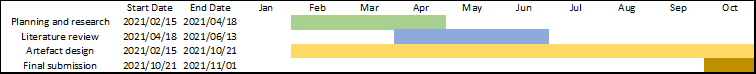
\includegraphics[scale=0.8]{Figures/Chart.png}
\caption{Project plan as represented by a Gantt chart}
\label{fig:fig1}
\end{figure}
\subsection{Scope and Limitations}
The scope for this project is the creating, testing, and computing accuracy of the model. Further research will have to be done in other projects at a later stage. The current limitations for this project is time as the deadline for the final presentations and artefact design is in November 2021. No other limitations with regards to financing or resources exists.\\\\
Risk analysis was conducted and all the risks involved are listed below:
\begin{itemize}
\item Model is not viable
\item Model is not accurate enough
\item Time is not enough to conclude research
\end{itemize}
\section{Development platform, resources, and environments}
Datasets: Still under procurement from third parties (AfriGIS, StatsSA, GeoTerra Image).\\
Operating system: Windows and Linux\\
Programming language: Python will be used\\
IDE: No specific. However current tools include Jupyter Notebooks, Google Colaboratory, and basic text editors.\\
The reason why these tools were chosen is for their versatility, ease of access, plethora of libraries and additional packages that can be imported as needed. 
\section{Ethical and legal implications}
The only legal and ethical implications for this project is in the form of third party data access. The ethics form is attached in Appendix \ref{AppendixA}
\section{Provisional chapter division}
Chapter 1 - Introduction\\
This will cover the outline of the project.\\
Chapter 2 - Literature Review\\
The focus of this section is to delve deeper into the relevant literature for this project and give a thorough analysis.\\
Chapter 3 - Artefact Design\\
The focus of this section will be on the complete processes involved in creating the model for this project.\\
Chapter 4 - Discussion\\
The focus in this section will be to analyse the results gained from the model and compare them to the relevant literature discussed before. Further assumptions and claims are also discussed here. Lastly, comparisons with other students' work will be discussed.\\
Chapter 5 - Conclusion\\
The research project is closed off and further insights for the future can also be given. Aim and objectives are re-examined to ensure if they were achieved.

% Chapter 2

\chapter{Literature Review} % Main chapter title

\label{Chapter2} % For referencing the chapter elsewhere, use \ref{Chapter1}

%----------------------------------------------------------------------------------------

% Define some commands to keep the formatting separated from the content

%----------------------------------------------------------------------------------------

\section{Cellular Automata and Game of Life}
Cellular Automata can be modelled in a number of dimensions including anything from one, two, three, four, or more dimensions.\citep{adamatzky2010game} In this project the focus will be on the two dimensional approach using a \textsl{n}-dimensional lattice (will be referred to as a grid). The grid can be of infinite size, however will be limited to a finite space i.e. a predetermined set of cells superimposed over a map of an informal settlement.\\\\
An individual square in the grid (which will be referred to as a cell) can have upto eight neighbours. This is shown in the diagram below.
\begin{figure}[H]
\centering
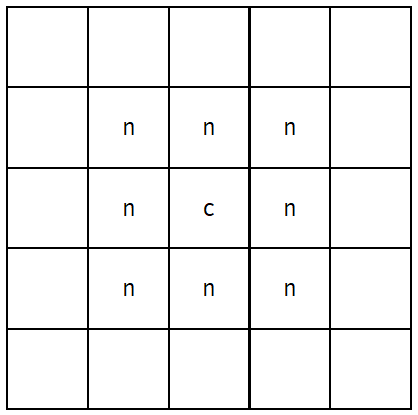
\includegraphics[scale=0.5]{Figures/Chapter2/cell.png}
\caption{A cell 'c' and its neighbours 'n'}
\label{fig:cell}
\begin{center}
Source: Own Creation (2021)
\end{center}
\end{figure}
A cell can have two discrete states for any given discrete time unit (referred to as generation). These states can be 'alive' or 'dead'. A cell is shown to be alive by having it \textsl{shaded} and if it is dead it is left blank.\citep{adamatzky2010game} This is shown in the figure below.
\begin{figure}[H]
\centering
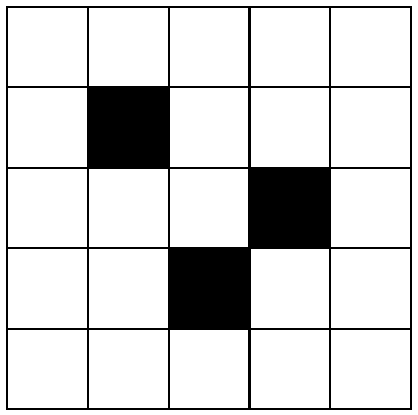
\includegraphics[scale=0.5]{Figures/Chapter2/shaded.png}
\caption{A grid showing alive and dead cells}
\begin{center}
Source: Own Creation (2021)
\end{center}
\end{figure}
As shown in Figure \ref{fig:cell} a cell can have either lateral or diagonal neighbours. The rules of \textsl{Life} were discussed briefly above in Section \ref{sec:prob}. A graphical representation of these is shown below.
\begin{figure}[H]
\centering
\begin{subfigure}{.5\textwidth}
  \centering
  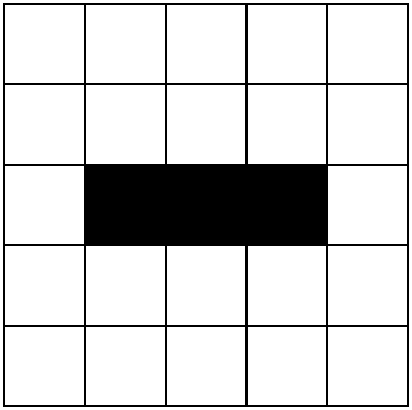
\includegraphics[width=.4\linewidth]{Figures/Chapter2/blink1.png}
  \caption{Generation $t = 0$}
\end{subfigure}%
\begin{subfigure}{.5\textwidth}
  \centering
  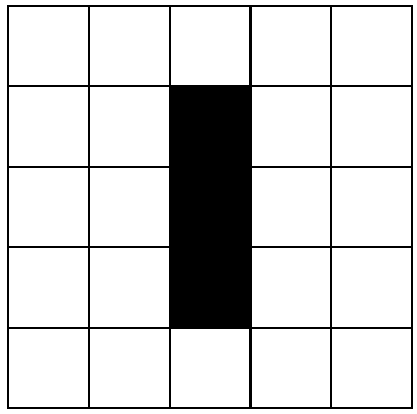
\includegraphics[width=.4\linewidth]{Figures/Chapter2/blink2.png}
  \caption{Generation $t = 1$}
\end{subfigure}
\caption{A simple 2 generation iteration of \textsl{Life}}
\begin{center}
Source: Own Creation (2021)
\end{center}
\end{figure}
Another slightly more advanced setup of \textsl{Life} is shown below.
\begin{figure}[H]
\centering
\begin{subfigure}{.5\textwidth}
  \centering
  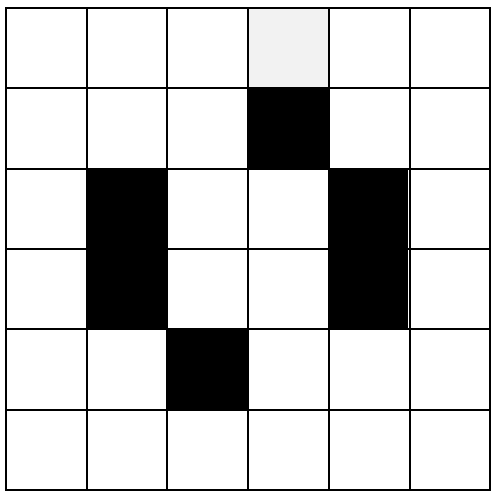
\includegraphics[width=.4\linewidth]{Figures/Chapter2/toad1.png}
  \caption{Generation $t = 0$}
\end{subfigure}%
\begin{subfigure}{.5\textwidth}
  \centering
  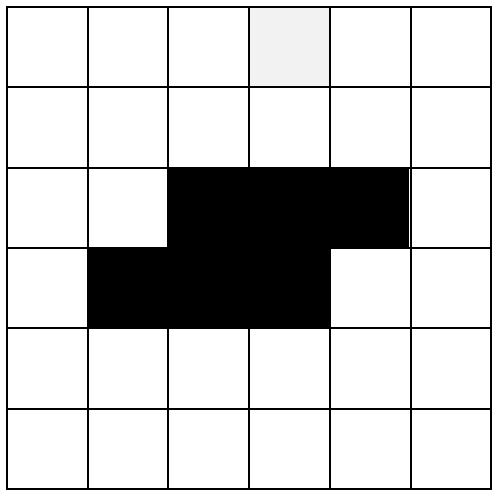
\includegraphics[width=.4\linewidth]{Figures/Chapter2/toad2.png}
  \caption{Generation $t = 1$}
\end{subfigure}
\caption{An advanced 2 generation iteration of \textsl{Life}}
\begin{center}
Source: Own Creation (2021)
\end{center}
\end{figure}
In a seminal paper by Stephen Wolfram, four classes of CA were proposed according to their behaviour given an initial random condition .\citep{Wolfram1984} These four classes are as follows:
\begin{itemize}
\item Class 1 - After a finite number of generations a unique homogeneous state is reached i.e. all cells become the same eventually.
\item Class 2 - Simple structures are generated which are either periodic, or stable (also called persistent).
\item Class 3 - An aperiodic (or chaotic) patterns emerge which carry on indefinitely.
\item Class 4 - Capable of universal computations i.e. can exhibit complex behaviour. 
\end{itemize}
Due to the nature of the rules of \textsl{Life} certain patterns emerge. This is thanks to the cycles of repeated stated which evolve over certain number of generations. These patterns include still-lifes, period two (or \textsl{blinkers}), gliders, oscillators, glider guns, and puffer trains.\citep{adamatzky2010game}

From Set Theory using a 2-Dimensional grid or an array the Adjacency of any two "squares" or "cells" in the grid can be defined as:\cite{aima}
\begin{center}
$\forall x, y, a, b$ \textit{Adjacent}$([x, y], [a, b])$\\\textit{if and only if}\\$(x = a \land (y = b - 1 \lor y = b + 1)) \lor (y = b \land (x = a - 1 \lor x = a + 1))$
\end{center}
Given a set of $[a, b]$ coordinates which can be defined in a 2-Dimensional grid or Cartesian plane with a corresponding to $x$ and $b$ corresponding to $y$. The $[a, b]$ values can then be changed according to rule specified. The Figure \ref{fig:ruleadj} below demonstrates this rule in a diagrammatical manner.
\begin{figure}[H]
\centering
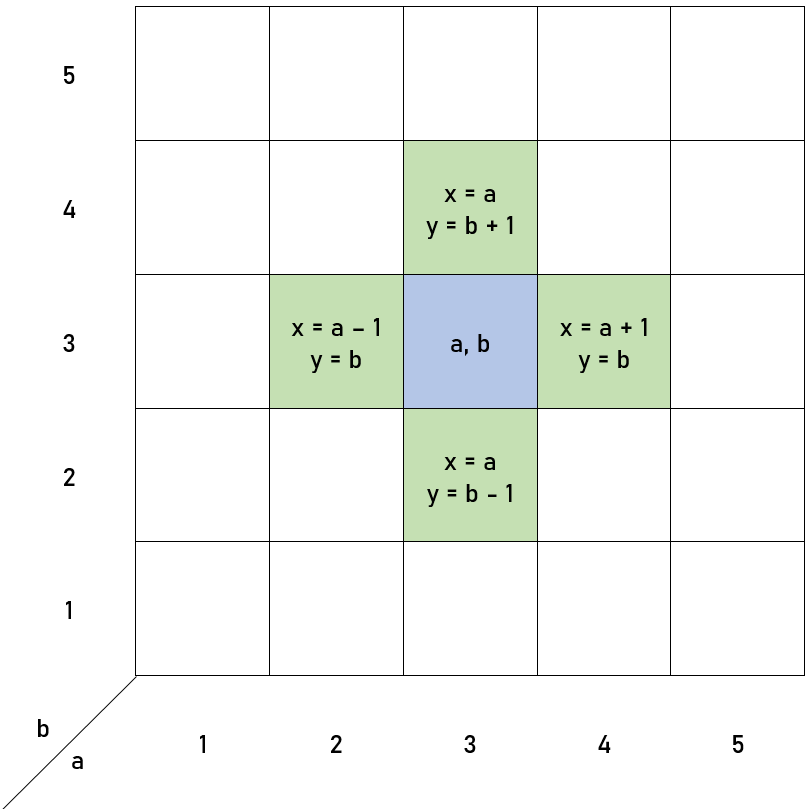
\includegraphics[scale=0.5]{Figures/Chapter2/adjacent}
\caption{Rule for Adjacency}
\label{fig:ruleadj}
\end{figure}
\begin{center}
Source: Own Creation (2021)
\end{center}
This configuration for the adjacency rule is known as the \textit{Von Neumann neighbourhood}\cite{ca}. The above rule from Set Theory can be expanded to include diagonal cells or blocks. The rule can be expanded as follows;
\begin{center}
$\forall x, y, a, b$ \textit{Adjacent}$([x, y], [a, b])$ \\ \textit{if and only if}\\$(x = a \land (y = b - 1 \lor y = b + 1)) \lor (y = b \land (x = a - 1 \lor x = a + 1))$\\ $\lor (x = a - 1 \land (y = b - 1 \lor y = b +1))$\\ $\lor (x = a + 1 \land (y = b - 1 \lor y = b + 1))$
\end{center}
This configuration for the adjacency rule is known as the \textit{Moore neighbourhood}\cite{ca}. The Figure \ref{fig:ruleadj2} below demonstrates this rule in a diagrammatical manner once again.
\begin{figure}[H]
\centering
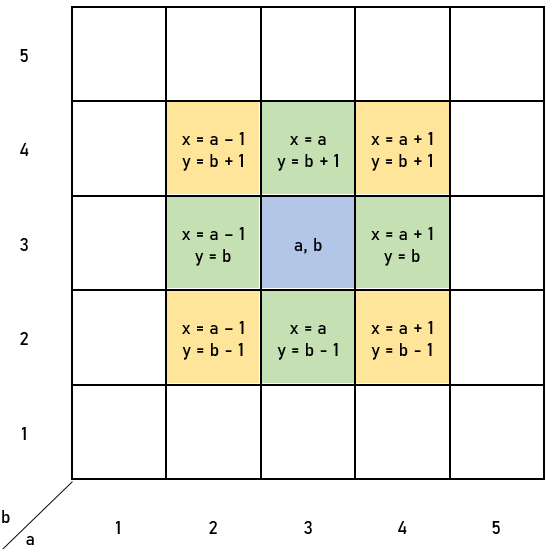
\includegraphics[scale=0.5]{Figures/Chapter2/adjacent2}
\caption{Rule for Adjacency Revised}
\label{fig:ruleadj2}
\end{figure}
\begin{center}
Source: Own Creation (2021)
\end{center}

The applications of CA and, or \textsl{Life} have sparked a number of research papers in fields such as physics, music, complexity, and computation. \\
Examples in physics include, interaction between a complex system and electromagnetic radiation \citep{conti}, an implementation of \textsl{Life} with quantum features.\citep{quantum}\\
Implementations in music include the development of CAMUS (\textbf{C}ellular \textbf{A}utomata \textbf{Mus}ic).\citep{music}\\
In the fields of complexity, and computation a vast array of work has been done therefore a few examples include; Universal Computer-Constructor in CA \citep{gou}, and creation of a Turing Machine in \textsl{Life}.\citep{ren}
\section{Informal settlements}
Informal settlements are housing dwellings that are part of urban districts or neighbourhoods that arise and develop without oversight or control from the state. They are synonymous with 'slums' or 'squatters', though are not the same. They form an integral element of urban sustainability whereby developing cities can not develop without them. The connotations with 'informal', 'slums', and 'squatter' have always been seen in a negative light. This is not seen as beneficial as the growth of urbanisation is highly intertwined with informal settlements.\citep{dovey2011forms}\\
Across the globe informal settlements are known colloquially by their own variety of terms. \citep{un} In this project the umbrella term informal settlement will be utilised.\\
The process or principles of informal settlements growth can be grouped into three categories namely;\citep{dovey2011forms}
\begin{itemize}
\item \textsl{settling} - simply settling down on what is usually unclaimed land
\item \textsl{inserting} - usually into urban areas that are abandoned, or uninhabited
\item \textsl{attaching} - informal settlements that grow out of existing urban settlements
\end{itemize}
In morphological terms, informal settlements can be classified into eight different types. This refers to the urban conditions rather that the process mentioned above, however it is not to say that the two are mutually exclusive. The types are not mutually exclusive from each other either. The types are as follows:\citep{dovey2011forms}
\begin{itemize}
\item Districts - most popular where over long periods of time the settlement grows to encompass mixed-use districts with both retail, and industrial functionality.
\item Waterfronts - settlements between land and water, whether it is a lake, harbour, river, canal to name a few. Prone to water issues such as flooding if the climate is such.
\item Escarpments - settlements on urban topography that is usually too steep to build formal structures. an example location would be an area between a mountain and a city. Can be prone to earthquakes, landslides, and mudslides if the climate is such. Transportation is another key concern.
\item Easements - Major infrastructure in urban cities such as roads, railways, pipelines to name a few offer \textsl{'buffer'} zones which can become informal settlements.
\item Sidewalks - These settlements emerge when public area such as sidewalks have an area where people can set up dwellings, even if for temporary usage.
\item Adherences - Related to the principle mentioned above.
\item Backstages - Settlements hidden from the public's gaze. Becomes more informal the \textsl{'deeper'} one goes from a formal street frontage.
\item Enclosures - Settlements where the \textsl{'shell'} is contained with in another urban building.
\end{itemize}
Informal settlement residents just like the residents of formal settlements have a desire for a good quality of life. Factors that influence this quality of life include food storage and preparation, water, sanitation, air quality and pollution, electricity, health risks, access to public facilities and amenities, among other things.\citep{richards2007measuring}\\
Richards et al. (2007), further sates that everyday problems such as unemployment, and crime also influence the quality of life. The paper further stipulates that the research can be expanded further to look into spatial and temporal factors that influence informal settlements.\\\\
The characteristics of informal settlements transcend the physical and are closely knitted with socio-economic as well as political conditions.\citep{wekesa}
\section{Modelling Urban Development}
\subsection{Historical Overview}
Historically, speaking humans have been pivoting between two standards namely; migrations and settlements. These standards have been driven by factors such as social, political, environmental, security, adventure to name a few.\cite{mum}

\subsection{Theories in Urban Planning}

The phenomenon of urbanisation in the last century has drastically increased from a mere 13\% in 1900 to a 49\% in 2005. The current projected estimates for the year 2030 in 60\%. The majority of this urbanisation is still going to occur in the developing nations.\citep{un2005}\\\\
One of the three factors that is going to influence humans directly in the near future is the land-use/land cover change. This will affect policy makers, geographers, and planners all alike. This is thanks to the socio–environmental consequences of the spatio-temporal process of urban development.\citep{vitousek1994beyond,liu2008modelling}\\\\
When it comes to geographic models they can be categorised into three categories of increasing abstraction.\citep{thomas1980modelling} The models are as follows:
\begin{itemize}
\item Scale
\begin{itemize}
\item Iconic
\item Analogue
\end{itemize}
\item Conceptual or Diagrammatical
\item Mathematical
\begin{itemize}
\item Probability
\item Deterministic 
\end{itemize}
\end{itemize}
The mathematical models are therefore the highest level of abstraction. Scale models mimic reality but are miniaturised copies of the real world. The main difference between Iconic and Analogue is the later besides being replicas they tend to transform certain properties of the real world system, e.g. using wool for clouds. Conceptual models are concerned with the relationships that exist between components in the system e.g. a sewage system can be denoted with arrows and boxes on a diagram. Mathematical models if in their purest form translate a conceptual model in to pure, formal, and symbolic logic of mathematics.\citep{thomas1980modelling}\\\\
The flow chart of the modelling process is shown below.
\begin{center}
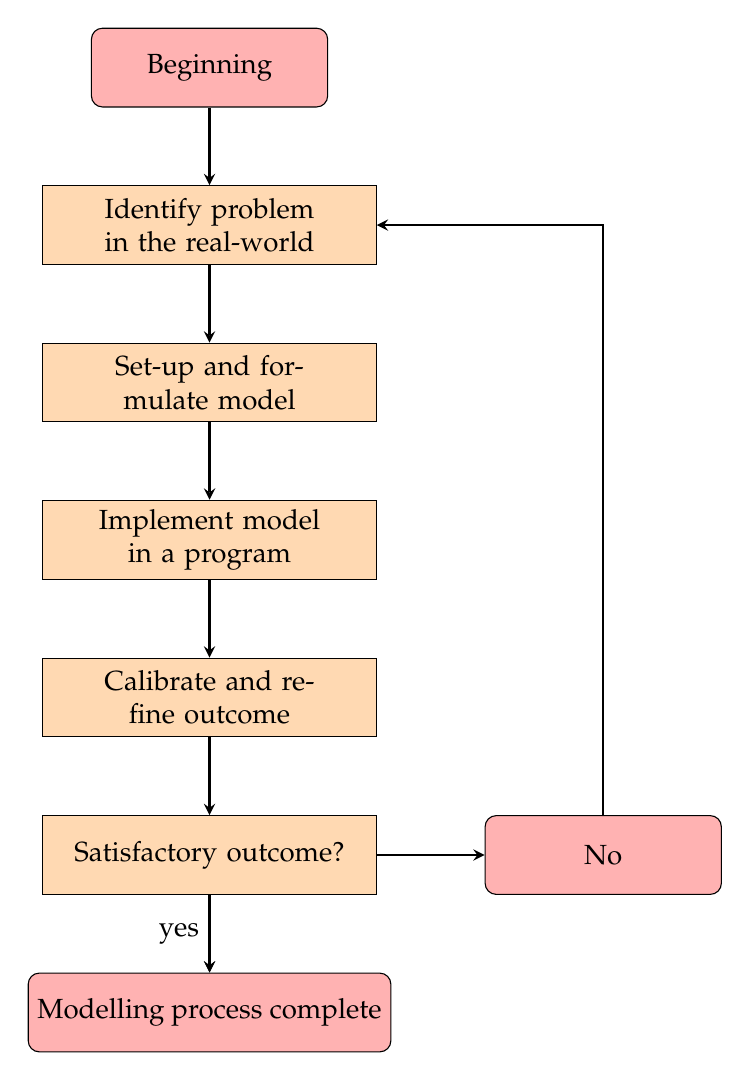
\begin{tikzpicture}[node distance=2cm]
\node (start) [startstop] {Beginning};
\node (pro1) [process, below of=start] {Identify problem in the real-world};
\node (pro2) [process, below of=pro1] {Set-up and formulate model};
\node (pro3) [process, below of=pro2] {Implement model in a program};
\node (pro4) [process, below of=pro3] {Calibrate and refine outcome};
\node (pro5) [process, below of=pro4] {Satisfactory outcome?};
\node (stop) [startstop, below of=pro5] {Modelling process complete};
\node (no) [startstop, right of=pro5, xshift=3cm] {No};
\draw [arrow] (start) -- (pro1);
\draw [arrow] (pro1) -- (pro2);
\draw [arrow] (pro2) -- (pro3);
\draw [arrow] (pro3) -- (pro4);
\draw [arrow] (pro4) -- (pro5);
\draw [arrow] (pro5) -- (stop);
\draw [arrow] (pro5) -- node[anchor=east] {yes} (stop);
\draw [arrow] (pro5) -- (no);
\draw [arrow] (no) |- (pro1);
\end{tikzpicture}
\\Source: Own Creation (2021) adapted from \citep{liu2008modelling}
\end{center}
Before continuing it should be noted that one of the major pitfalls of models are they are a simplified view of reality, hence they can tend to leave certain facts behind of reality.\citep{liu2008modelling}\\\\
One of the earliest models created in geography and urban modelling dates back to the 1800s where Johann Heinrich von Th{\"u}nen in his book titled \textsl{Der isolierte Staat} translated to mean \textsl{The Isolated State} discussed maximising agricultural production.\citep{clark1967thunen}

Other seminal research included the like of Alfred Weber in the early 1900s published the title \textsl{{\"U}ber den Standort der Industrien} which translates to \textsl{Theory of the Location of Industries}. This work created models based on real-world conditions.\citep{fearon2006alfred}

The seminal work on the three classical models of urban structure, growth, and urban land usage patterns was done by a number of authors. The models include Concentric Zone Theory, Sector model, and the Multiple nuclei model.\citep{liu2008modelling}
These models laid the foundations for later computer based models to emerge in the field of urban modelling. The early works include techniques on simulation, linear analysis, and mathematical programming.\citep{kilbridge1970population}
Among the first studies carried out on simulations of real-world cases using urban CA was done by \citep{batty}.

The meta-analysis carried out by Sante et al. (2010) showed that a number of characteristics are utilised in each of the studies that resulted in a varied range of accuracy for the models implemented in CA for urban growth.\citep{ca1}
A few characteristics are:
\begin{itemize}
\item Cell space
\item States
\item CA relaxations (Neighbourhood, Transition rules, Constraints)
\item Calibration
\item Validation
\end{itemize}
Additional factors were also implemented which also helped in creating a
varied range of accuracies. Some of these factors include:
\begin{itemize}
\item Accessibility of transport
\item Distance to railways, airports, and urban centres
\item Social services
\item Slope \& Elevation
\item Environmental factors
\item Hazard lands
\item Agricultural value
\item Urban suitability
\item Zoning
\item Population density
\item Land value
\item Construction year
\item Water supply
\item Social housing
\end{itemize}
All of the above with a combination of additional research will now help the
project move to the next step which is the development of the artefact, which
in this project's case is a model.
\section{Geographic Information Systems and its Data}

ArcGIS API for Python\footnote{\url{https://pro.arcgis.com/en/pro-app/latest/arcpy/get-started/arcgis-api-for-python.htm}}
\\\\
ArcGIS API for Python is a Python library for performing GIS visualization and analysis, spatial data management, and GIS system administration tasks that can run both in an interactive fashion and using scripts.
\\\\
It enables power users, system administrators, and developers to leverage the SciPy ecosystem for automating their workflows and performing repetitive tasks using scripts. It integrates well with the Jupyter Notebook and enables academics, data scientists, GIS analysts, and visualization enthusiasts to share geoenriched literate programs and reproducible research.
\\\\
The online overview describes how to use ArcGIS API for Python to write Python scripts, incorporating capabilities such as mapping, query, analysis, geocoding, routing, portal administration, and more. Browse the sample notebooks to get started.
\\\\
GitHub\footnote{\url{https://github.com/Esri/arcgis-python-api}}
\\\\
What is ArcPy?\footnote{\url{https://pro.arcgis.com/en/pro-app/latest/arcpy/get-started/what-is-arcpy-.htm}}
ArcPy is a Python site package that provides a useful and productive way to perform geographic data analysis, data conversion, data management, and map automation with Python.

This package provides a rich and native Python experience offering code completion (type a keyword and a dot to get a pop-up list of properties and methods supported by that keyword; select one to insert it) and reference documentation for each function, module, and class.

The additional power of using ArcPy is that Python is a general-purpose programming language. It is interpreted and dynamically typed and is suited for interactive work and quick prototyping of one-off programs known as scripts while being powerful enough to write large applications in. ArcGIS applications written with ArcPy benefit from the development of additional modules in numerous niches of Python by GIS professionals and programmers from many different disciplines.

ArcPy (often referred to as the ArcPy site package) provides Python access for all geoprocessing tools, including extensions, as well as a wide variety of useful functions and classes for working with and interrogating GIS data. Using Python and ArcPy, you can develop an infinite number of useful programs that operate on geographic data.
\\\\
QGIS API Documentation\footnote{\url{https://qgis.org/api/}}
\\\\
QGIS Python API Documentation\footnote{\url{https://qgis.org/pyqgis/3.10/}}
\\\\
The CORE library contains all basic GIS functionality\\
The GUI library is build on top of the CORE library and adds reusable GUI widgets\\
The ANALYSIS library is built on top of CORE library and provides high level tools for carrying out spatial analysis on vector and raster data\\
The SERVER library is built on top of the CORE library and adds map server components to QGIS\\
The 3D library is build on top of the CORE library and Qt 3D framework\\
Contains classes related to implementation of QGIS plugins\\
The QgsQuick library is built on top of the CORE library and Qt Quick/QML framework
\section{Images and Colour Theory}
\label{sec:col}
sfsdfs \cite{imgp} Image processing
image thresholding \cite{shap}  
% Chapter 3

\chapter{Artefact Design \& Development} % Main chapter title
\label{Chapter3} % For referencing the chapter elsewhere, use \ref{Chapter3}
\section{Description of Artefact}
The nature of the research that is conducted in this study leads to a contrasting artefact that is delivered. The artefact is a culmination of image processing, programming, GIS data handling, and problem solving. This is made obvious as this chapter progresses further. In essence the artefact is the steps and procedures followed to come up with the final CA model.
\section{Life Cycle Methodology}
\label{sec:lcm}
For the entire development of the Artefact a combination of three methodologies was utilised. These included:
\begin{itemize}
\item Waterfall
\item Agile
\item Scrum
\end{itemize}
The rationale for utilising this combination was due to the following factors:
\begin{itemize}
\item The emphasis on self-management for the design and development of the Artefact.
\item Incremental changes made in short iterations.
\item Segmenting problems into workable pieces and thereafter completing them in an effective manner.
\item Analysing and recording each stage of the research progress and evaluating the progress to prevent backsliding.
\item Iteratively solving smaller issues and problems as they arise.
\end{itemize}
\section{Design Science Schema for Research Study}
According to Gregor \& Hevner, 2013 there are seven sections involved in tackling a Research study. They are listed as follows:\cite{dssteps}
\begin{enumerate}
\item Introduction
\item Literature Review
\item Method
\item Artifact Description
\item Evaluation
\item Discussion
\item Conclusions
\end{enumerate}
In conjunction with the methodologies discussed in Section \ref{sec:lcm} this research study will incorporate the Design Science Schema as follows:
\begin{itemize}
\item Chapter \ref{Chapter1} of this research study will fall under Step 1.
\item Chapter \ref{Chapter2} of this research study will fall under Step 2.
\item Chapter \ref{Chapter3} of this research study will fall under Steps 3, 4 and 5.
\item Chapter \ref{Chapter4} of this research study will fall under Step 6.
\item Chapter \ref{Chapter5} of this research study will fall under the last Step 7.
\end{itemize}
\section{Data Acquisition}
\subsection{Closed Sourced Data}
After the Literature Review was conducted the search for data began. A company by the name of GeoTerraImage (Pty) Ltd\footnote{\url{https://geoterraimage.com/}} which is located in Pretoria, South Africa was contacted and a data request was filed. The GIS data received was for an Informal settlement named \textit{"Melusi"}. The author is grateful for the data provided. The dataset received contained three main points of interest to this research:
\begin{itemize}
\item The outline or boundary of the \textit{"Melusi"} area.
\item The Building Based Land Usage in the form of housing for the year 2010 for \textit{Melusi}.
\item The Building Based Land Usage in the form of housing for the year 2020 for \textit{Melusi}.
\end{itemize}
\subsection{Open Sourced Data}
\label{sec:open}
To assist with the CA modelling additional data was needed. The following two websites  were utilised:
\begin{itemize}
\item The Humanitarian Data Exchange\footnote{\url{https://data.humdata.org/}}
\item The South African Department of Water and Sanitation\footnote{\url{https://www.dwa.gov.za/}}
\end{itemize}
From the above mentioned websites the following GIS data was acquired:
\begin{itemize}
\item All the medium-scale river coverage in South Africa.\footnote{\url{https://www.dws.gov.za/iwqs/gis_data/river/rivs500k.aspx}} This dataset was in the \texttt{.SHP} format.
\item All the Road networks in South Africa provided by HOTOSM (Humanitarian OpenStreetMap Team) and available for download by HDX (The Humanitarian Data Exchange).\footnote{\url{https://data.humdata.org/dataset/hotosm_zaf_roads}} This dataset was in the \texttt{.SHP} format.
\item High Resolution Population Density Maps \& Demographic Estimates in South Africa in the year 2019 which was once again made available for download by HDX.\footnote{\url{https://data.humdata.org/dataset/cbfc4206-35c8-42d4-a096-b2dd0aec983d}} This dataset was in the \texttt{.TIF} format.
\end{itemize}
\section{Data Exploration and Preprocessing}
\subsection{Usage of Geographic Information Systems}
\label{sec:GIS}
The use of Geographic Information Systems (GIS) was not greatly successful in this research. The factors limiting the usage were; the lack of packages, libraries, add-ons, or plug-ins that function "out-of-the-box", the ones that do work tend to fulfill niched application or specific problems.

Additional issues encountered were as follows:
\begin{itemize}
\item Incompatibility of Operating Systems.
\item GIS data formats were incompatible.
\item Researchers publising their Masters or Doctorates research made custom tools that were specific to their research.
\end{itemize}
The following GIS tools were utilised in the early stages of the research:
\begin{itemize}
\item ESRI's ArcGIS (Proprietary commercial software).\footnote{\url{https://www.esri.com/en-us/home}}
\item QGIS (Open-source software).\footnote{\url{https://qgis.org/en/site/}}
\end{itemize}

The following packages, libraries, add-ons, or plug-ins were also utilised in the early stages of the research:
\begin{itemize}
\item MOLUSCE - A plugin for QGIS for Land Use Change Evaluation.\footnote{\url{https://wiki.gis-lab.info/w/Landscape_change_analysis_with_MOLUSCE_-_methods_and_algorithms}}
\item TerraME - A Multiparadigm Modeling Toolkit.\footnote{\url{http://www.terrame.org/doku.php}}
\item GeoSOS (Geographic Simulation \& Optimization System) - A standalone program or as an add-on for ArcGIS.\footnote{\url{https://www.geosimulation.cn/GeoSOS/}}
\end{itemize}
These endeavours were also unfruitful with the reasons being the same as mentioned above.

It should be noted that the above packages do have CA modelling capabilities but were limited. The author embarked on creating his own model.

Lastly, another key hurdle was the availability of some tools which required the use of programming languages that were out of the scope of this author's skill set.

The dataset that were acquired up until this point had to analysed, therefore the next logical step was to load the GIS data into the GIS software to provide a quick overview.
\subsection{Handling of GIS Data in GIS Software}
The datasets were loaded first into ArcGIS and thereafter into QGIS. The figures below demonstrate the output achieved.
\begin{figure}[H]
\centering
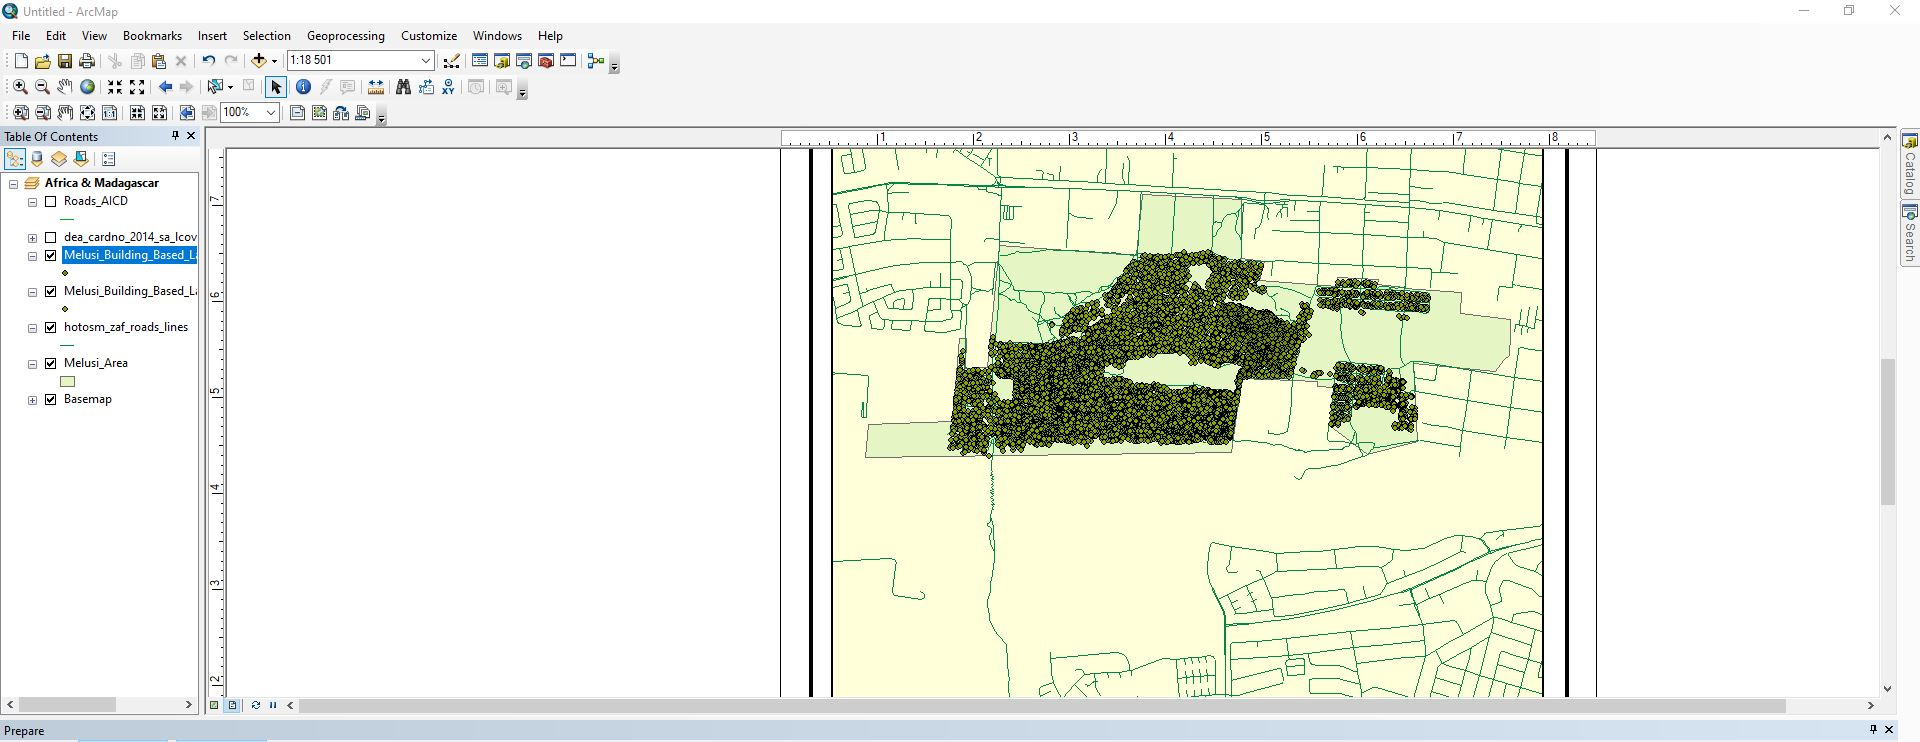
\includegraphics[scale=0.3]{Figures/Chapter3/ArcGIS}
\caption{Output of the datasets in ArcGIS}
\label{fig:Arc}
\end{figure}
\begin{figure}[H]
\centering
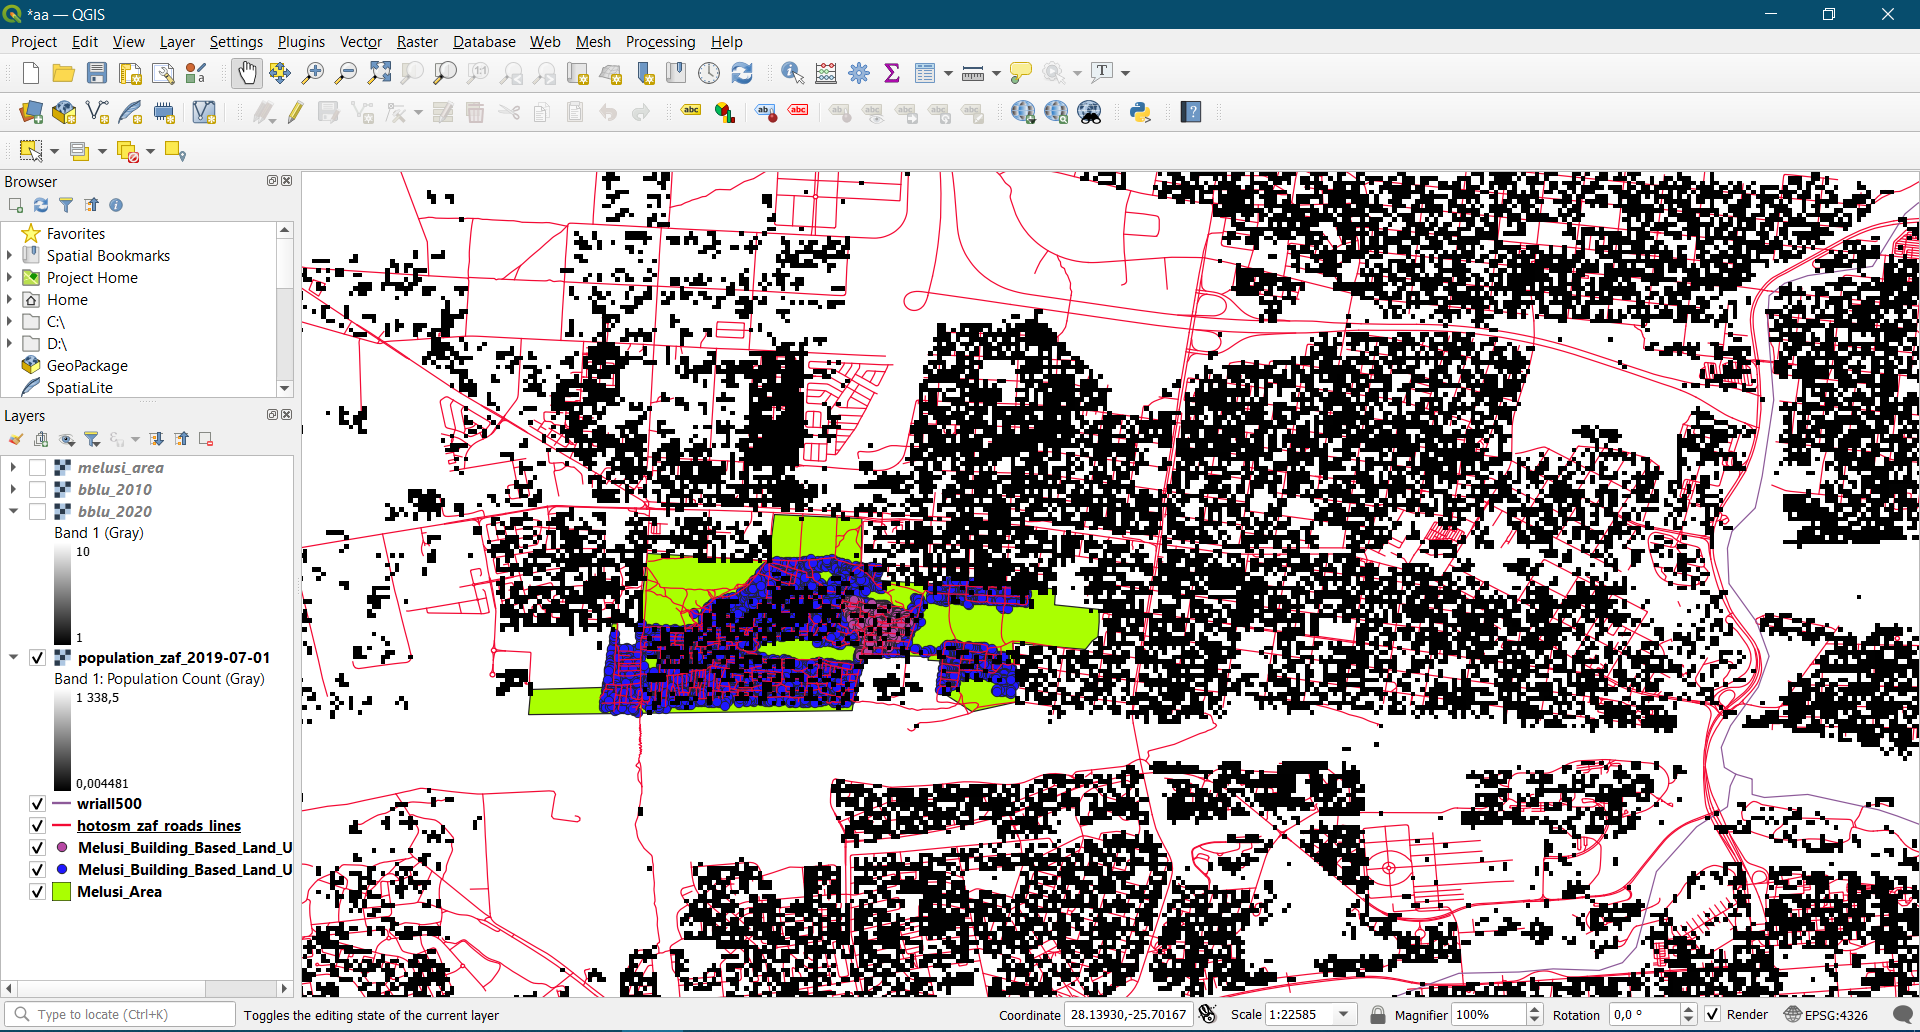
\includegraphics[scale=0.35]{Figures/Chapter3/QGIS}
\caption{Output of the datasets in QGIS}
\label{fig:Q}
\end{figure}
In the Figure \ref{fig:Arc} where ArcGIS is shown, the dark green colour represent Building Based Land Usage in the year 2020, however the Land Usage for the year 2010 was blended inside the bigger Building Based Land Usage of 2020. The lighter green colour represents the roads network in the year 2019.

In the next Figure \ref{fig:Q} where QGIS is shown, the black colour represents the population dataset, the light green colour represents the boundary of the \textit{Melusi} area. The blue colour represents the Building Based Land Usage for the year 2010, and the purple colour is the Building Based Land Usage for the year 2020. Lastly, the light pink colour represents the roads network in the year 2019.

At this juncture the dataset for the medium-scale river coverage was dropped from the research as both the GIS software indicated that there was not any rivers close by  in the area.

As was mentioned in Section \ref{sec:GIS} this was the limit of the GIS software usage in this research. The next approach was to utilise the Python programming language as well as its vast array of libraries.
\subsection{Handling of GIS Data with Python}
\begin{figure}[H]
\centering
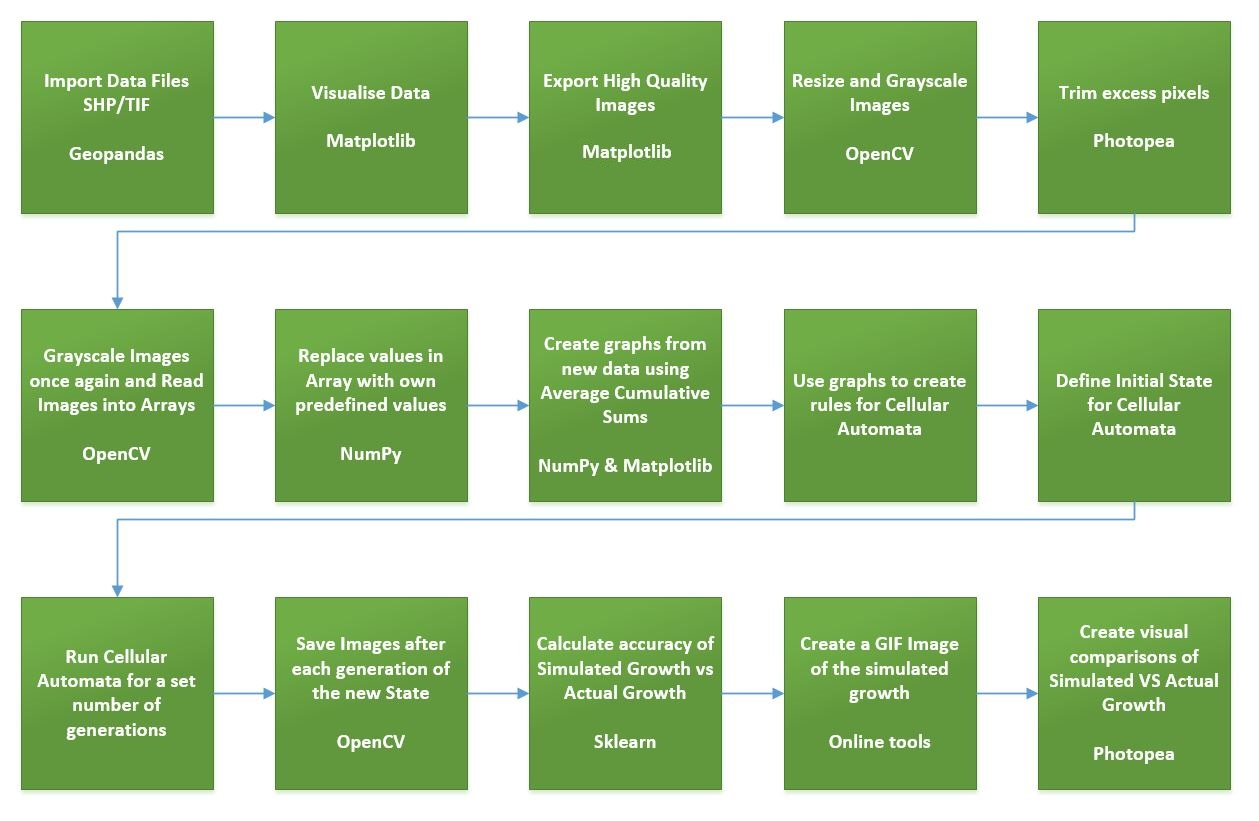
\includegraphics[width=1\textwidth]{Figures/Chapter3/Overview}
\caption{A high-level overview of Python use in this research}
\end{figure}
The primary approach used with Python was the use of Python Notebooks. These were run in two different environments:
\begin{itemize}
\item Locally using Jupyter Notebook.\footnote{\url{https://jupyter.org/}}
\item On the cloud using Google Colaboratory.\footnote{\url{https://research.google.com/colaboratory/}}
\end{itemize}
Jupyter Notebook utilises the local resources an individual has on a computer to run Python code.

Google Colab is an example of Platform as a Service (PaaS), and Infrastructure as a Service (IaaS) combined into one service.

PaaS is a cloud service model which supports application development in the cloud using languages and other tools. IaaS on the other hand is cloud service model which offers network components, storage, and processing in the cloud.\cite{pf} These service models do not require users to have powerful computing components as it is "outsourced" to these vendors such as Google.

Therefore, the only requirement for Google Colab is to utilise a modern browser that is capable of opening the Colab website to run Python code.
\\\\
The Geopandas\footnote{\url{https://geopandas.org/}} and the Matplotlib\footnote{\url{https://matplotlib.org/}} libraries were utilised to load the datasets and carry out elementary visual analysis. Additionally, the library called Folium\footnote{\url{https://python-visualization.github.io/folium/}} was utised to create an interactive map to demonstrate the boundaries of \textit{Melusi} in repect to other surrounding regions.

The first dataset to be loaded was the \textit{Melusi} dataset which had the \texttt{.SHP} files. This was done using the Geopandas \texttt{read\_file} method.\footnote{\url{https://geopandas.org/docs/reference/api/geopandas.read_file.html}}\\\\
From the Folium library the \texttt{map} method\footnote{\url{https://python-visualization.github.io/folium/modules.html\#module-folium.map}} was utilised after the coordinates were extracted from the data loaded into Geopandas and visualisations were made using Matplotlib. The \texttt{pyplot.plot} method\footnote{\url{https://matplotlib.org/stable/api/_as_gen/matplotlib.pyplot.plot.html\#matplotlib.pyplot.plot}} was used for this step.

Below are a few figures that were created in this process. The coordinates of this region can also be seen in the figures above.
For more information on these steps involved, the Appendix \ref{AppendixC} has more details.
\begin{figure}[H]
\centering
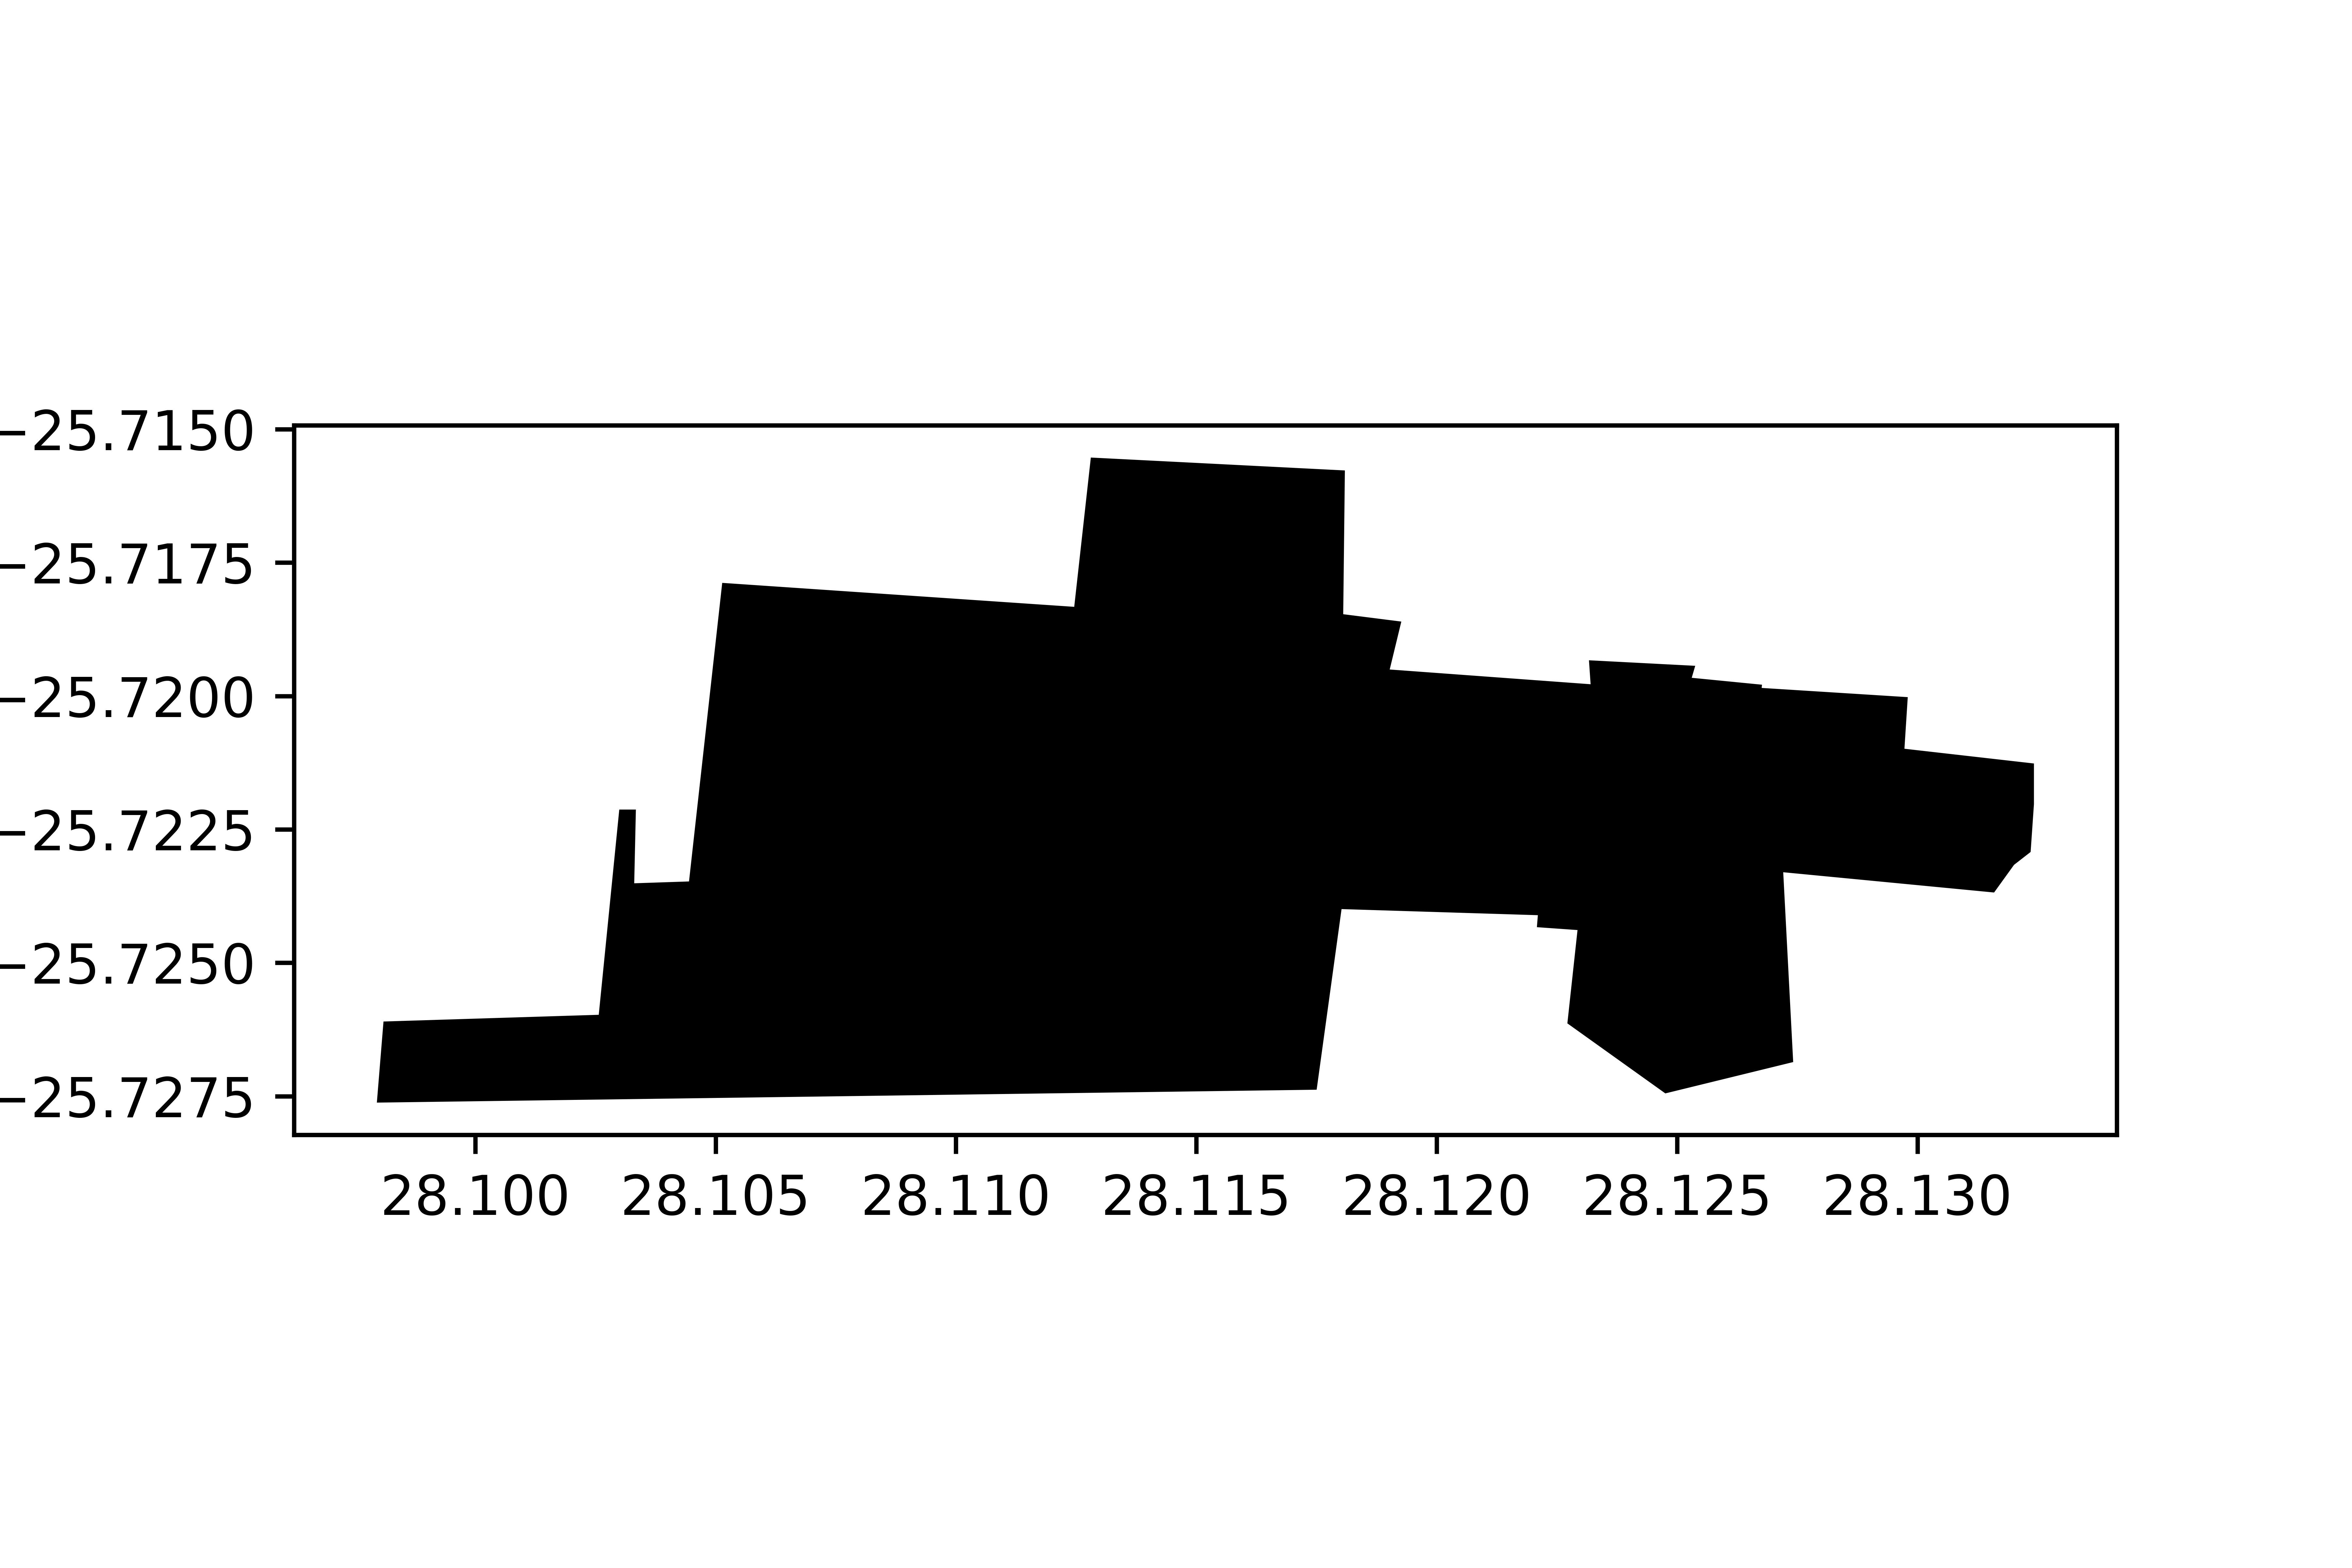
\includegraphics[width=1\textwidth]{Figures/Chapter3/MelusiArea}
\caption{The boundary of the \textit{Melusi} area}
\end{figure}
\begin{figure}[H]
\centering
\includegraphics[width=1\textwidth]{Figures/Chapter3/Melusi2010}
\caption{The Building Based Land Usage of the \textit{Melusi} area in 2010}
\label{fig:mel2010}
\end{figure}
\begin{figure}[H]
\centering
\includegraphics[width=1\textwidth]{Figures/Chapter3/Melusi2020}
\caption{The Building Based Land Usage of the \textit{Melusi} area in 2020}
\label{fig:mel2020}
\end{figure}
Once the coordinates were acquired the Folium interactive map was created of the \textit{Melusi} area. This is shown at the endof this Chapter in Figures \ref{fig:fol} and \ref{fig:fol2}. The surrounding suburbs and regions can also be seen. The webpages for these can be accessed here\footnote{\url{https://github.com/AM-ops/Hons-Project-Documentation/blob/main/Hons-Project-Documentation-Final/Web/melusi_area.html}}$^{,}$\footnote{\url{https://github.com/AM-ops/Hons-Project-Documentation/blob/main/Hons-Project-Documentation-Final/Web/melusi_area2.html}}
The file can be downloaded and thereafter viewed interactively in a browser.

The Building Based Land Usage for 2010 and 2020 can be seen in Figures \ref{fig:mel2010} and \ref{fig:mel2020}

After the above \textit{Melusi} area datasets were explored the next two variables needed to be explored. These were the road networks and the population datasets.

The road networks dataset as was mentioned in Section \ref{sec:open} is in the \texttt{.SHP} format, therefore once again the Geopandas \texttt{read\_file} method was employed to read the data. However the population dataset was in the \texttt{.TIF} format therefore another library Rioxarray had to be utilised.\footnote{\url{https://corteva.github.io/rioxarray/stable/rioxarray.html}} The method from this library is to read the file is \texttt{open\_rasterio}.

Data that is loaded using Geopandas is stored in \texttt{GeoDataFrames} whereas the data loaded using Rioxarray is stored in \texttt{DataArrays}. Each of these data structures have different methods and properties that allow for the manipulation of the data. This is demonstrated below.

In the next procedure the following has to be kept in mind; the aforementioned two datasets contain data for the entirety of South Africa, therefore they have to be limited to just the \textit{Melusi} area. To accomplish this firstly, the \textit{Melusi} area's boundary was extracted using the \texttt{GeoSeries.total\_bounds} property\footnote{\url{https://geopandas.readthedocs.io/en/latest/docs/reference/api/geopandas.GeoSeries.total_bounds.html}} provided by Geopandas.

Thereafter, this boundary limit was applied to the data structures mentioned earlier. This is done through the \texttt{cx} property\footnote{\url{https://geopandas.org/docs/reference/api/geopandas.GeoDataFrame.cx.html}} from Geopandas and was applied to the road networks \texttt{GeoDataFrame}. The \texttt{rio.clip\_box} method\footnote{\url{https://corteva.github.io/rioxarray/stable/_modules/rioxarray/raster_array.html\#RasterArray.clip_box}} from Rioxarray was applied to the population \texttt{DataArray}.

Matplotlib was once again employed for plotting purposes. The resulting images for the population and road networks datasets is shown in Figures \ref{fig:popgraph} and \ref{fig:roadgraph}.
\begin{figure}[H]
\centering
\includegraphics[width=1\textwidth]{Figures/Chapter3/Roads2019}
\caption{The Road Networks in the \textit{Melusi} area as of 2019}
\label{fig:roadgraph}
\end{figure}
\begin{figure}[H]
\centering
\includegraphics[width=1\textwidth]{Figures/Chapter3/Population2019}
\caption{The Population Density of the \textit{Melusi} area as of 2019}
\label{fig:popgraph}
\end{figure}
%ax = roads.plot(color="black", figsize=(7,5))
%ax.set\_axis\_off()
%ax.set(xlim=(xmin, xmax), ylim=(ymin, ymax))
%ax.autoscale\_view(scalex=False, scaley=False)
%ax.autoscale(enable=False)
%ax.autoscale(enable=False)
%plt.savefig("roads-nox.jpg",dpi=1200)
The next process involved exporting or saving high quality images of all the figures shown above namely; Figures \ref{fig:mel2010}, \ref{fig:mel2020}, \ref{fig:roadgraph}, and \ref{fig:popgraph}. A 2-Dimensional grid or lattice is needed for a CA model hence the need to export the images. An image is in essence a 2-Dimensional grid whereby the width and height is predefined and any pixel in the image can be referenced using a 2-Dimensional co-ordinate system.

The pixel density (known as Dots Per Inch or DPI)\cite{dpi} was set to 1,200 and the Matplotlib library's \texttt{pyplot.savefig}\footnote{\url{https://matplotlib.org/stable/api/_as_gen/matplotlib.pyplot.savefig.html}} method was called to save all the images. Additionally, the axes were set to be turned off\footnote{\url{https://matplotlib.org/3.1.1/api/_as_gen/matplotlib.axes.Axes.set_axis_off.html}} and, the autoscale\footnote{\url{https://matplotlib.org/3.1.1/api/_as_gen/matplotlib.pyplot.autoscale.html}} for figures was set to \texttt{False}.\\\\
Before the images were saved a few key aspects had to be verified. The first was making sure the Coordinate Reference System (CRS) was the same for all the datasets involved. The approach for \texttt{GeoDataFrames} is to call the \texttt{crs} property\footnote{\url{https://geopandas.org/docs/reference/api/geopandas.GeoDataFrame.crs.html}} and for the \texttt{DataArrays} the \texttt{rio.crs} accessor\footnote{\url{https://corteva.github.io/rioxarray/stable/getting_started/crs_management.html}} can be accessed.

The CRS for all the datasets was \textit{EPSG 4326}, therefore the process of saving the images was done immediately without the need for the CRS for any dataset to be changed.
\subsection{Image Processing with OpenCV}
\label{sec:imgproc}
After the images above were saved and analysed the following final dimensions were achieved, thanks to the high DPI;
\begin{itemize}
\item Width: 7,200 px
\item Height: 4,800 px
\end{itemize}
To assist in the CA modelling (discussed further down) and to simplify the process, one of the approached that can be taken is to scale the images (also known as resizing). Another approach is to grayscale the images. Both of these approaches were applied. The rationale behind using these approaches is as follows; A trade off can be made between computational time in modelling with the data loss in an image.\cite{impact} Additionally, the norm in Image Processing Modelling is to utilise Convolutional Neural Networks, this will not be the approach taken in this research.\cite{cnn}

With regards to grayscaling, and fields such as image recognition the method or type of algorithms utilised to grayscale color images does impact performance.\cite{gray} However in this research those finer details are not in the project scope, hence a basic grayscale operation was performed for all of the following images:
\begin{itemize}
\item Building Based Land Usage of the \textit{Melusi} area in 2010.
\item Building Based Land Usage of the \textit{Melusi} area in 2020.
\item Road networks of the \textit{Melusi} area in 2019.
\item Population Density of the \textit{Melusi} area in 2019.
\end{itemize}

The grayscale operation was carried out using the Python version of the OpenCV library\footnote{\url{https://docs.opencv.org/4.x/}}. The conversion from a RGB image to grayscale is done with the \texttt{cvtColor} method\footnote{\url{https://docs.opencv.org/3.4.15/de/d25/imgproc_color_conversions.html}}

The grayscale formula from OpenCV's Documentation is as follows:
\begin{center}
$\text{RGB[A] to Gray:} \quad Y \leftarrow 0.299 \cdot R + 0.587 \cdot G + 0.114 \cdot B$
\end{center}
This formula simplified means the Red value of a pixel is multiplied with 0.299, the Green value of the pixel is multiplied with 0.587, and lastly the Blue value of a pixel is multiplied with 0.114. These new three values are summed up to give one value for the pixel in grayscale.

The first three images listed above do not differ greatly visually as they are mainly white and black to start of with. Therefore, the Population Density image is ideal to demonstrate the output of the grayscale operation. Below in Figure \ref{fig:popogray} the output is visualised.
\begin{figure}[H]
\centering
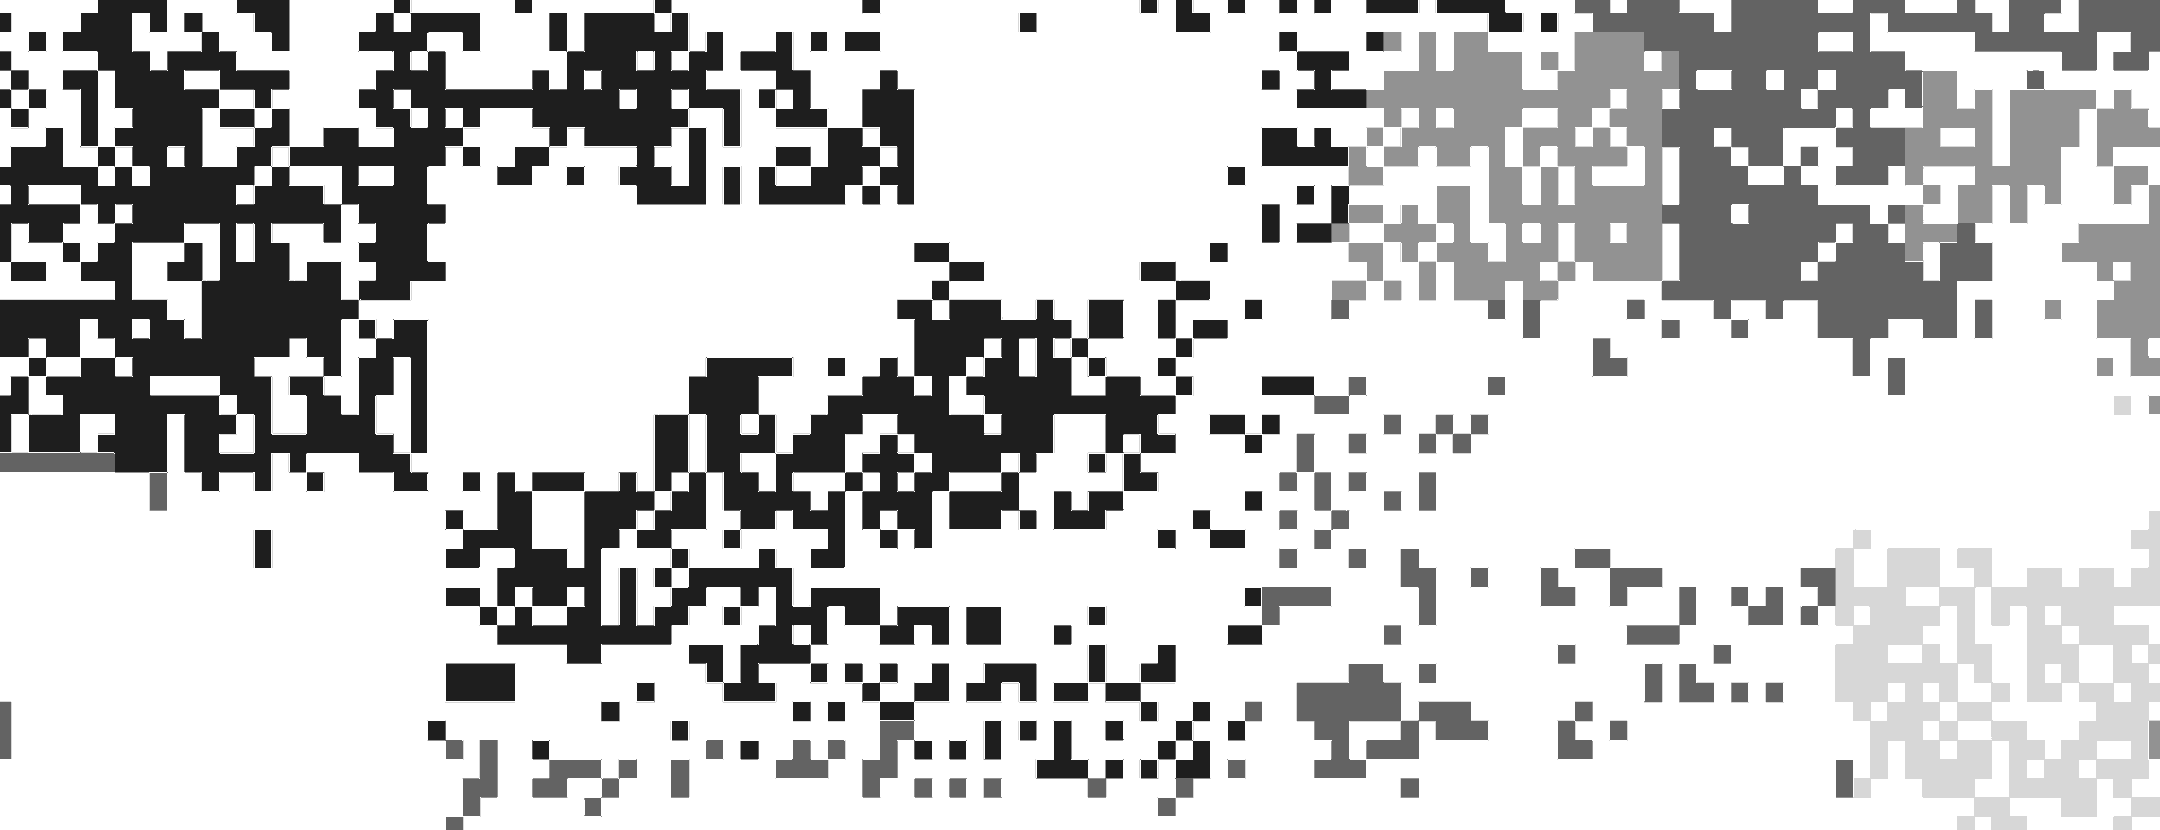
\includegraphics[width=1\textwidth]{Figures/Chapter3/popgray}
\caption{The grayscale image from the Population Density data}
\label{fig:popogray}
\end{figure}
Additionally, the process of scaling the images utilised the \texttt{resize} method\footnote{\url{https://docs.opencv.org/3.4.15/da/d54/group\_\_imgproc\_\_transform.html\#ga47a974309e9102f5f08231edc7e7529d}} which was called. The scale factor was $\frac{1}{3}$. This scale factor was chosen to prevent excess data. At this stage the Data Preprocessing is complete and the only aspect remaining is to to save the images after being processed. For this the \texttt{imwrite} function\footnote{\url{https://docs.opencv.org/4.x/d4/da8/group__imgcodecs.html\#gabbc7ef1aa2edfaa87772f1202d67e0ce}} from OpenCV was called for each of the four final images.

Thereafter, the Online Photo Editor, Photopea\footnote{\url{https://www.photopea.com/}} was employed to trim some of the edges of the images. The resulting dimensions of the images were as follows:
\begin{itemize}
\item Width: 2,160 px
\item Height: 830 px
\end{itemize}
These resulting dimensions were ideal for the next process which involved creating the CA model.
\section{Cellular Automata Modelling}
\subsection{Preliminary Discussion}
To begin the process of creating the CA model, the first step involves reading the final images created from the steps in Section \ref{sec:imgproc}. This once again requires the use of OpenCV. The function employed is the \texttt{imread} function\footnote{\url{https://docs.opencv.org/4.x/d4/da8/group__imgcodecs.html\#ga288b8b3da0892bd651fce07b3bbd3a56}}.

Once the images are read into variables the grayscale function has to be applied again. This is due to the nature of the \texttt{imwrite} function which saves images in the RGB format. This is also true for images that where grayscaled before and saved.

The \texttt{imread} function returns a \texttt{ndarray} also know as a NumPy N-Dimensional Array. In the case of Images the \texttt{ndarray} is a 2-Dimensional Array. Using NumPy's Indexing\footnote{\url{https://numpy.org/doc/stable/reference/arrays.indexing.html\#arrays-indexing}} (Slicing) capabilities one can effortlessly access any value in the \texttt{ndarray}. The images needed for the modelling process are read into separate variables and the next procedures can be carried out.
\\\\
At this juncture the 2-Dimensional grids for the CA model are ready in the form of \texttt{ndarrays}. The images which are read into \texttt{ndarrays} are ready for a custom thresholding. As was expanded in Section \ref{sec:col}, thresholding is an additional approach that makes the process of defining rules for the CA modelling slightly more elementary. The two \texttt{ndarrays} that are put through the thresholding process are:
\begin{itemize}
\item The Population Density
\item The Road Networks
\end{itemize}
For the Population Density array all the unique values were extracted using the NumPy \texttt{unique} Set routine. The Table \ref{table:uniq} below shows the output of these values.
\begin{table}[H]
\caption{Unique values found in the population \texttt{ndarray}}
\label{table:uniq}
\centering
\begin{tabular}{@{}l@{}}
\toprule
\multicolumn{1}{c}{Unique Values} \\ \midrule
0.5483527804562259                \\
1.9322995070209252                \\
2.494171667535703                 \\
2.5802248275941975                \\
2.928383276590716                 \\
3.843662634917949                 \\
3.9742969374931736                \\
4.0719211311237515                \\
5.236094447939968                 \\
5.558666899272438                 \\
NaN                               \\ \bottomrule
\end{tabular}
\end{table}
From this table the function \texttt{replaceWithPopulationDensity} was created. The details of this can be found in Appendix \ref{AppendixC}.

For the Roads a simpler threshold function was created which was called \texttt{replaceRoadsForCalc}. The basic principle for this function is to replace all pixels in the array with a 1 if it is black (Meaning a road is present at that pixel) or white otherwise (no road present). The details can once again be found in Appendix \ref{AppendixC}.

These custom functions that were created utilised the NumPy \texttt{vectorize} function\footnote{\url{https://numpy.org/doc/stable/reference/generated/numpy.vectorize.html}} to be applied to the entire arrays. The rationale for using \texttt{vectorize} is increased computational speed in carrying out the functions.

Another custom function that utilses \texttt{vectorize} is the \texttt{replaceBWForCalculations}. This function is exactly the same as the \texttt{replaceRoadsForCalc}, however it is used in the course of the CA model's simulation runtime. As the name suggests it replaces Black and White pixels with 1s and 0s in the Building Based Land Usage array.

The Roads array and the Population array which are vectorized, from here on will be labelled as \textit{variable arrays}. The two Building Based Land Usage arrays, which are not yet vectorized will be labelled as \textit{State arrays} due to them having states in the CA model simulation.

At this point all the four arrays which are synonymous with the four images saved in Section \ref{sec:imgproc} should be kept in mind as a 2-Dimensional array or grid on which a CA model can be created and simulated. The Figure \ref{fig:gridlayers} shows a diagrammatical visualisation of three identical (with regards to width and height) 2-Dimensional data arrays. The figure demonstrates that referencing a specific block or cell within these grid would be the same in any of them.
\begin{figure}[H]
\centering
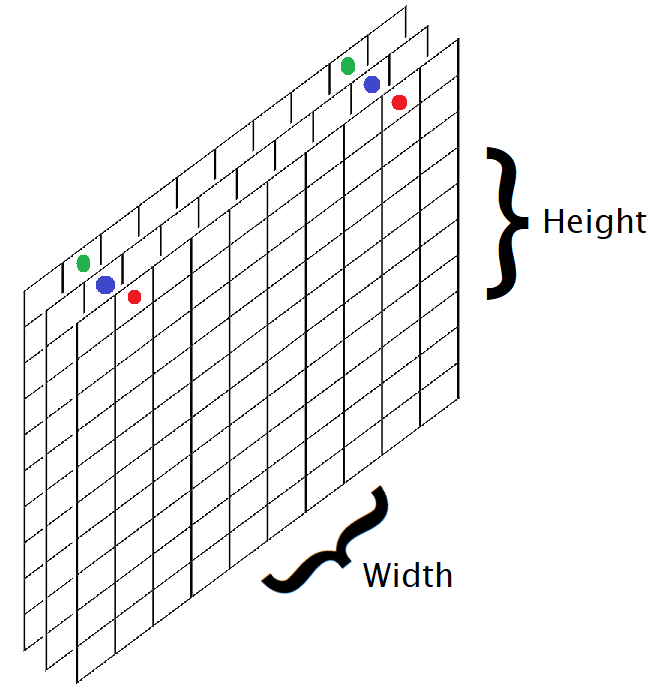
\includegraphics[scale=0.6]{Figures/Chapter3/gridlayers}
\caption{Multiple Identical 2D Arrays visualised}
\label{fig:gridlayers}
\end{figure}
The next logical step is to formulate rules for the CA Model. However before this can be conducted, the Rule of Adjacency from Section \ref{sec:LitCA} can be discussed further. The reason for this is to manage any and all edge cases that may arise while creating the rules for the CA model.

Additionally, the method of referencing blocks based on location should be uniform, therefore below in Figure \ref{fig:labs} the naming conventions for this research are specified. These are also the labels which are used in the code located in Appendix \ref{AppendixC}. 
\begin{figure}[H]
\centering
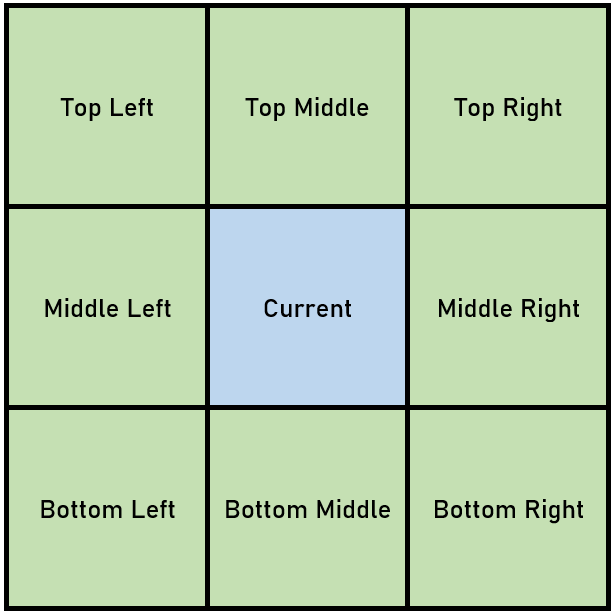
\includegraphics[scale=0.5]{Figures/Chapter3/labels}
\caption{Naming conventions for neighbours}
\label{fig:labs}
\end{figure}
The avant-garde approach which in turn is also intuitive to solve the issues of edge cases is to visualise two separate 2-Dimensional arrays. The first is of size $3 \times 3$ (labelled as $A$), and the the other is $n \times n$ (labelled as $B$) where $n$ is of arbitrary value. Thereafter, assign the center block of grid $A$ as the \textit{Current} or \textit{Active} cell, and any of the other neighbouring cells as the edge case to be tested. Place the \textit{Current} cell on top of grid $B$ and align it with the top-left cell of grid $B$. Keeping the grid $B$ static begin to move grid $A$ towards the right-hand side of the grid $B$. Take note of the cells where the current edge case being tested fails. In other words, the edge case's cell lies outside of the grid $B$. All the edge cases can therefore be managed in any grid of size ($n \times n$) if the procedure is followed correctly. In the Figures \ref{fig:e1}, \ref{fig:e2}, \ref{fig:e3}, and \ref{fig:e4} this avant-garde process is demonstrated visually. The colours in the pictures are defined below:
\begin{itemize}
\item Green - \textit{Current} or \textit{Active} Cell
\item Grey - Neighbours of \textit{Current} Cell not being tested at the moment
\item Red - Edge case being tested.
\item Blue - Locations where edge case (in Red) passes
\item White - Locations where edge case (in Red) fails 
\end{itemize}

\begin{figure}[H]
\centering
\begin{subfigure}{.4\textwidth}
  \centering
  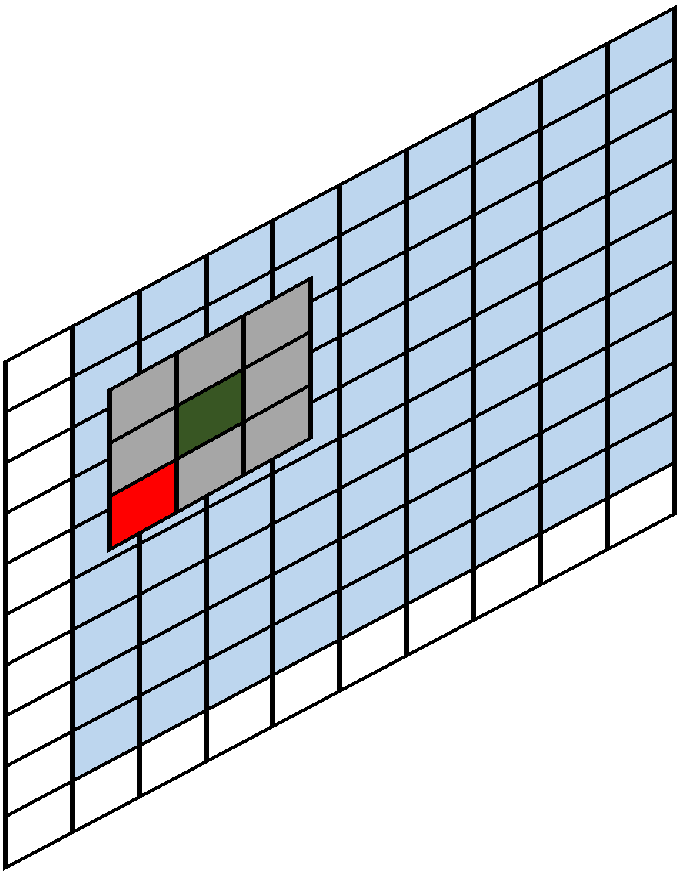
\includegraphics[width=.5\linewidth]{Figures/Chapter3/botleft}
  \caption{Bottom Left Cell}
\end{subfigure}%
\begin{subfigure}{.4\textwidth}
  \centering
  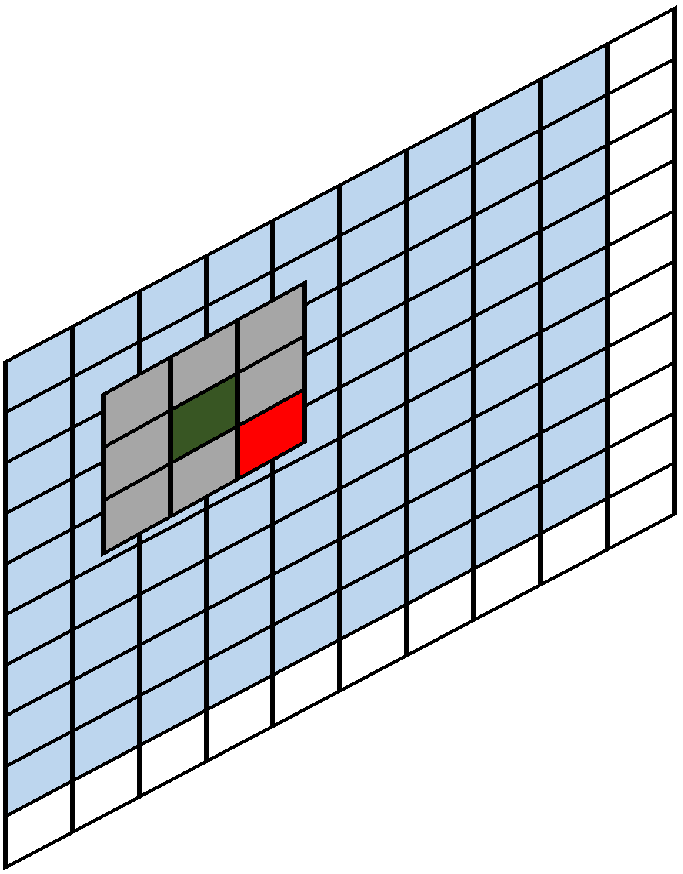
\includegraphics[width=.5\linewidth]{Figures/Chapter3/botright}
  \caption{Bottom Right Cell}
\end{subfigure}
\caption{Edge cases for Bottom Diagonal Cells}
\begin{center}
Source: Own Creation (2021)
\end{center}
\label{fig:e1}
\end{figure}

\begin{figure}[H]
\centering
\begin{subfigure}{.4\textwidth}
  \centering
  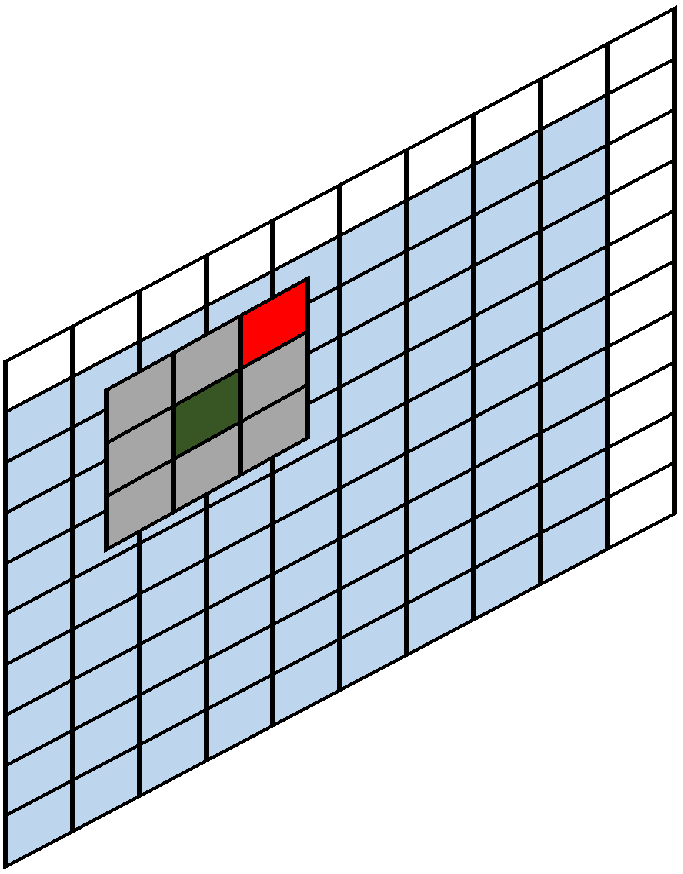
\includegraphics[width=.5\linewidth]{Figures/Chapter3/topright}
  \caption{Top Right Cell}
\end{subfigure}%
\begin{subfigure}{.4\textwidth}
  \centering
  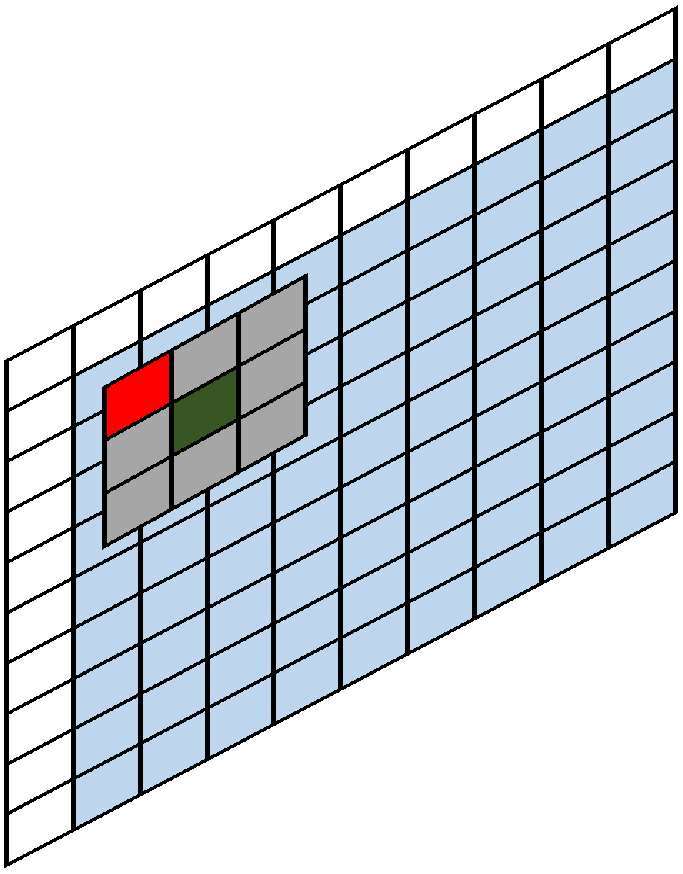
\includegraphics[width=.5\linewidth]{Figures/Chapter3/topleft}
  \caption{Top Left Cell}
\end{subfigure}
\caption{Edge cases for Top Diagonal Cells}
\begin{center}
Source: Own Creation (2021)
\end{center}
\label{fig:e2}
\end{figure}

\begin{figure}[H]
\centering
\begin{subfigure}{.4\textwidth}
  \centering
  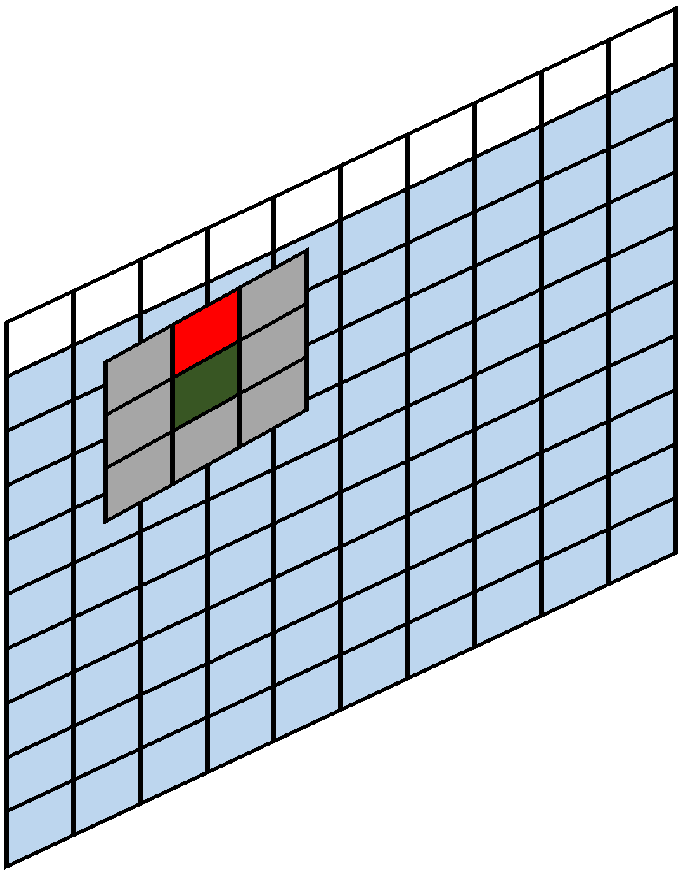
\includegraphics[width=.5\linewidth]{Figures/Chapter3/topmid}
  \caption{Top Middle Cell}
\end{subfigure}%
\begin{subfigure}{.4\textwidth}
  \centering
  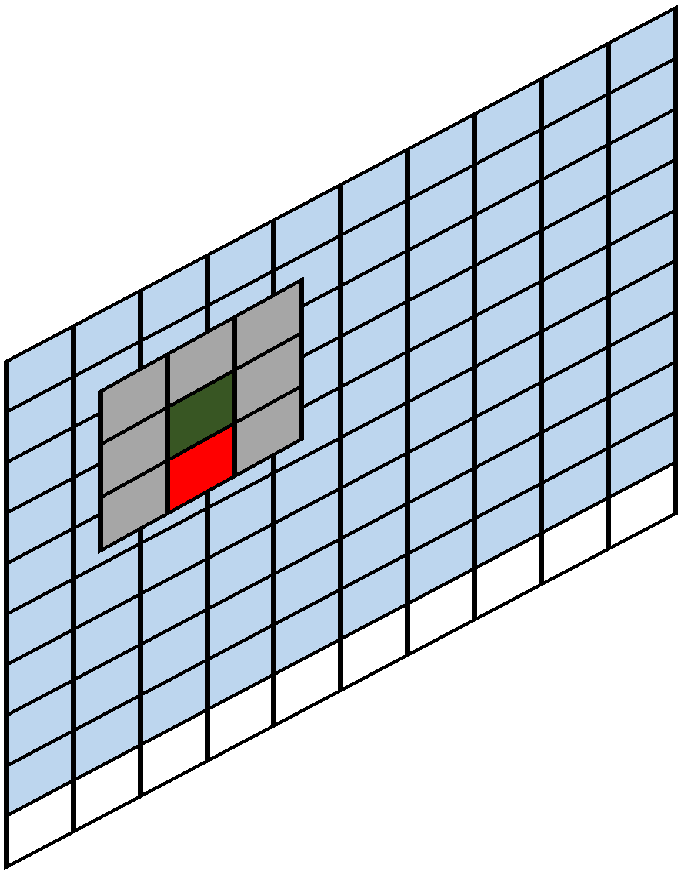
\includegraphics[width=.5\linewidth]{Figures/Chapter3/botmid}
  \caption{Bottom Middle Cell}
\end{subfigure}
\caption{Edge cases for Middle Column Cells}
\begin{center}
Source: Own Creation (2021)
\end{center}
\label{fig:e3}
\end{figure}

\begin{figure}[H]
\centering
\begin{subfigure}{.4\textwidth}
  \centering
  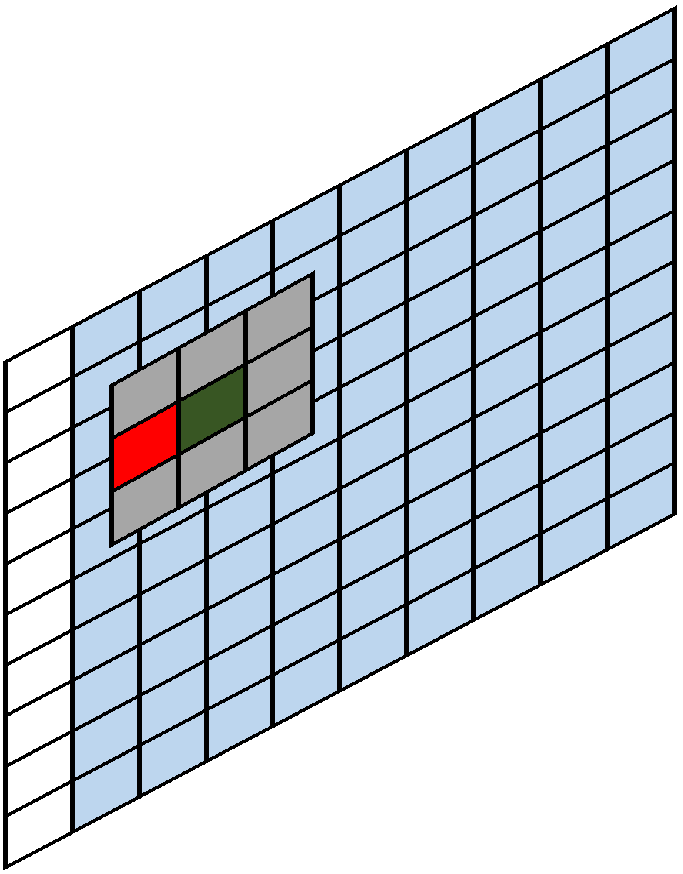
\includegraphics[width=.5\linewidth]{Figures/Chapter3/midleft}
  \caption{Middle Left Cell}
\end{subfigure}%
\begin{subfigure}{.4\textwidth}
  \centering
  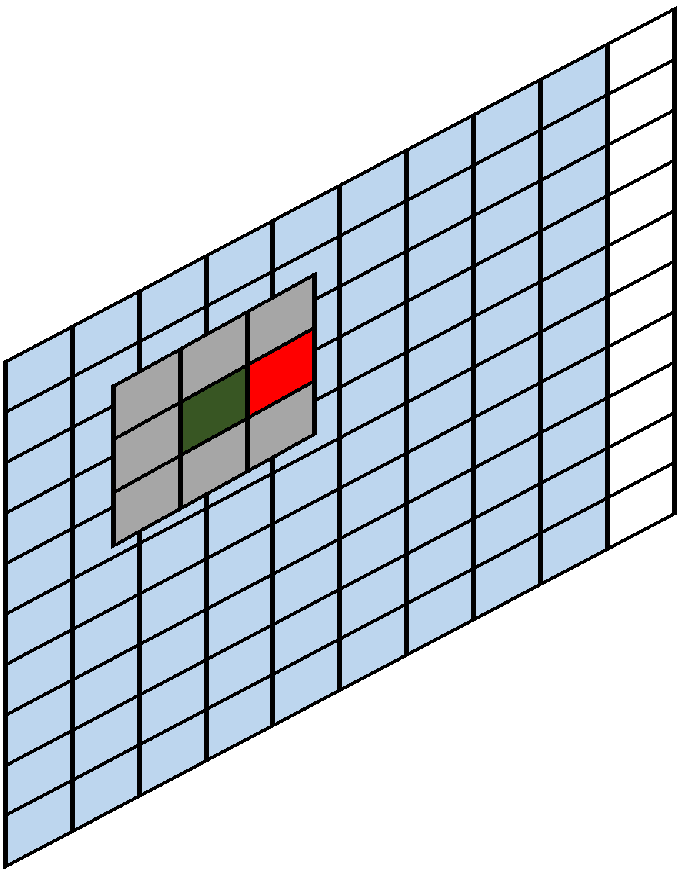
\includegraphics[width=.5\linewidth]{Figures/Chapter3/midright}
  \caption{Middle Right Cell}
\end{subfigure}
\caption{Edge cases for Middle Row Cells}
\begin{center}
Source: Own Creation (2021)
\end{center}
\label{fig:e4}
\end{figure}
The rationale behind this lengthy and detail process is due to the following reasons:
\begin{itemize}
\item The CA model must not throw any errors while it iterates through the grid
\item The next step which involves formulating growth rules for the CA model contains the process of splitting the original 3 arrays into $10 \times 10$ sized smaller arrays. This translates to a $10 \times 10$ pixel block in the final images.
\end{itemize}
\subsection{Formulation of Rules}
Referring back to the information provided in Section \ref{sec:imgproc}, the reasoning for having images in the dimensions of 2,160 px by 830 px is clear. These images which are now called \textit{variable arrays} when they are assigned to variables (after being read)  will have the same 2-Dimensional size, hence the step of splitting the variable arrays into smaller subsets is simplified without being wary of outlying values. The grid size for the CA model is therefore in the dimensions of $2,160 \times 830$ elements. The individual cells dimensions in this grid are $10 \times 10$, therefore the total cells present is:
\begin{center}
$216 \times 83 = 17,928$
\end{center}
The concept of Pooling was discussed in Section \ref{sec:col}, the different rules that can be applied to down-size inputs was also touched upon. The Figure \ref{fig:pool} demonstrated the Max rule which returns the maximum value from a given set, however for this research study the summing and averaging approach is employed. The detailed procedure is discussed below.

The Cumulative Sum of all individual cells in the variable arrays is taken. This means a total of 35,856 Cumulative Sums are carried out ($17,928 + 17,928 = 35,856$ for the two variable arrays). To calculate this sum the NumPy \texttt{cumsum} routine\footnote{\url{https://numpy.org/doc/stable/reference/generated/numpy.cumsum.html}} was called. Thereafter each of the Cumulative Sums is divided by $100$ to get the Average Cumulative Sum. This is because each cell in the variable arrays has $10 \times 10 = 100$ values.

The Figure \ref{fig:cumsumpool} below demonstrates an example of a Cumulative Sum Pool Operation which is carried out for each of the cells in the variable arrays. This operation sums all the values found in a given cell. The averages of each these sums (35,856 in total) is easily calculated thereafter.
\begin{figure}
\centering
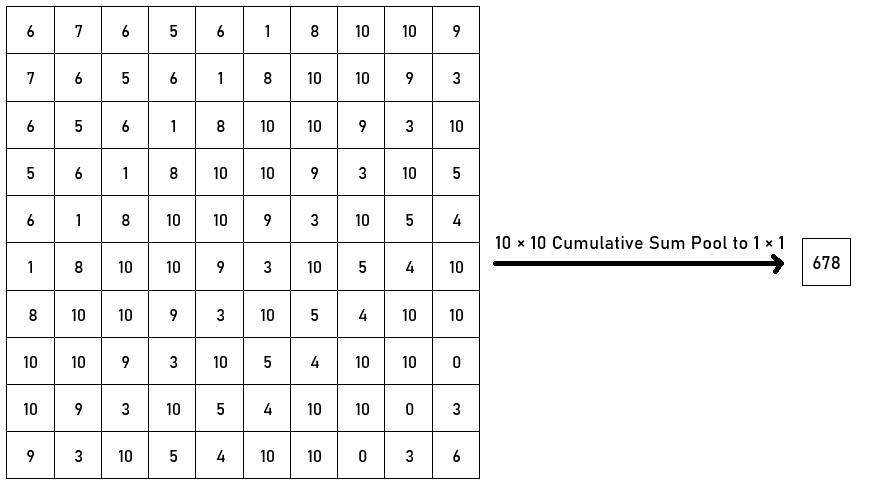
\includegraphics[scale=0.7]{Figures/Chapter3/sumpool}
\caption{An example of a \textit{Cumulative Sum Pool Operation}}
\label{fig:cumsumpool}
\end{figure}
After the averages of the Cumulative Sums is carried out the frequency of said averages is visualised to analyse the spread of the occurring values. This is then used to formulate conditional rules for the CA model. The Figures \ref{fig:cumsumpop} and \ref{fig:cumsumroad} below display the results of the visualisations.
\begin{figure}[H]
\centering
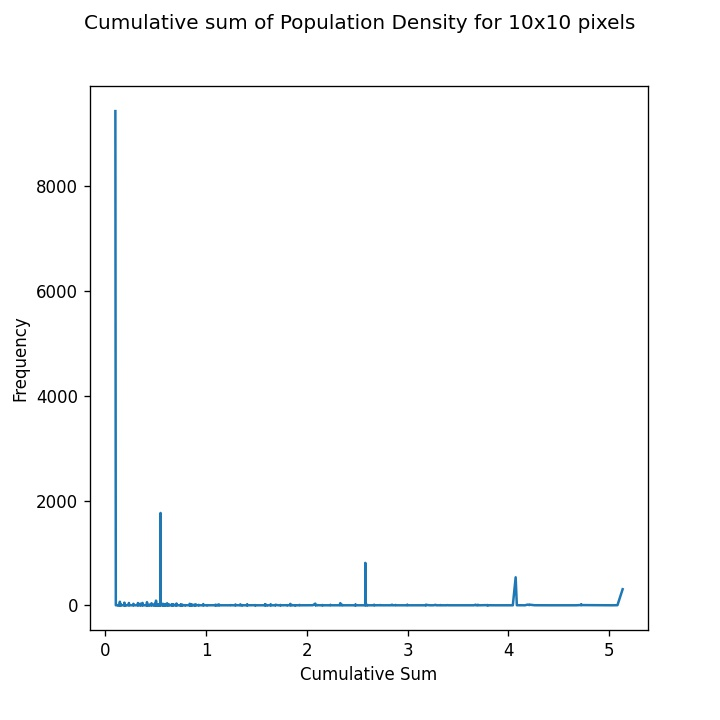
\includegraphics[scale=0.7]{Figures/Chapter3/populationSum}
\caption{Frequency of Averages of the Cumulative Sums in the Population variable array}
\label{fig:cumsumpop}
\end{figure}
\begin{figure}[H]
\centering
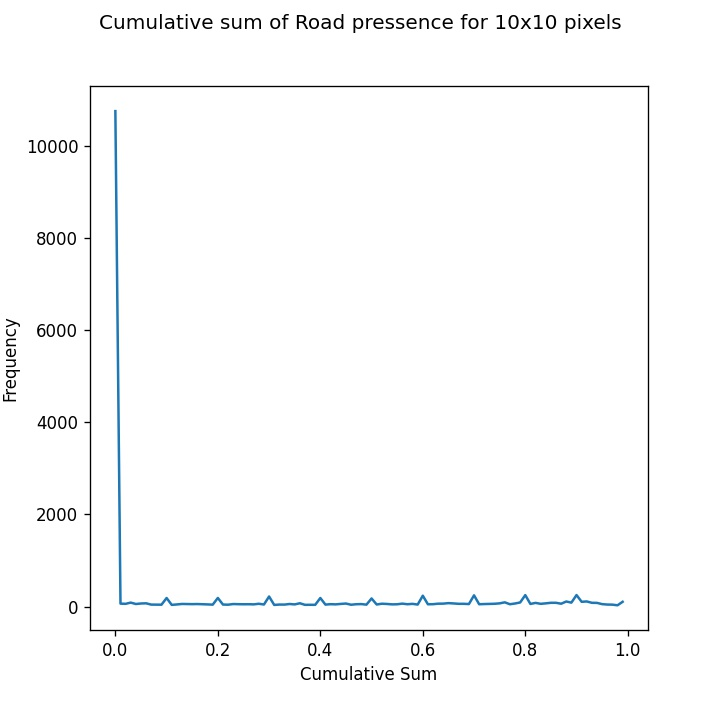
\includegraphics[scale=0.7]{Figures/Chapter3/roadsSum}
\caption{Frequency of Averages of the Cumulative Sums in the Roads variable array}
\label{fig:cumsumroad}
\end{figure}
\subsection{Cellular Automata Model in Operation}
\label{sec:runmod}
The first step before executing the model is to create an Initial State. This was set to the Building Based Land Usage array of 2010. The 2020 array is assigned the Final State. A Temporary copy of the Initial State is also created.

Thereafter the model is run for a total of 50 time periods. In each time period the model begins at the top-left cell of the Initial State and works its way through the entire grid. The cumulative sum operations are calculated for the current cells neighbours and the neighbours in the identical locations in the variable array. The averages thereafter are calculated to determine if the These predefined set of conditional rules as mentioned in the previous section are satisfied. If the conditional rules were satisfied the current cell where the model had reached in the current time period would be 'filled' in by converting all the pixel values of the Temporary array to black. Once a time period is completed the Initial State array is updated by using the Temporary array's 'filled' in values. This prevents unnecessary changes from happening during the modelling process.

The following two steps are carried out before moving on to the next time period.
\begin{enumerate}
\item Calculate the accuracy of the current Initial State to the Final State. This is done by flattening both the Building Based Land Usage arrays and thereafter running the \texttt{cohen\_kappa\_score} metric\footnote{\url{https://scikit-learn.org/stable/modules/generated/sklearn.metrics.cohen_kappa_score.html}} from the Scikit-learn library. Lastly, save the accuracy results.
\item Write the current Initial State to a new image with a name corresponding to the time period it was created in.

The final conditional rules that were settled on for the CA model are described in the Table \ref{table:rules} below.
\begin{table}[H]
\caption{Final rules for the Cellular Automata Model}
\label{table:rules}
\begin{tabular}{@{}lcccc@{}}
\toprule
\multicolumn{1}{c}{Time period (t)} & \begin{tabular}[c]{@{}c@{}}Population\\ Condition (p)\end{tabular} & \begin{tabular}[c]{@{}c@{}}Roads\\ Condition (r)\end{tabular} & \begin{tabular}[c]{@{}c@{}}Diagonal\\ Averages (d)\end{tabular} & \begin{tabular}[c]{@{}c@{}}Non-Diagonal\\ Averages (n)\end{tabular} \\ \midrule
t = 1                               & 0                                                                  & 0                                                             & 0                                                               & 0                                                                   \\
t = 2                               & 0                                                                  & 0                                                             & 0                                                               & 0                                                                   \\
t = 40                              & 0                                                                  & 0                                                             & 0                                                               & 0                                                                   \\
t = 50                              & 0                                                                  & 0                                                             & 0                                                               & 0                                                                   \\ \bottomrule
\end{tabular}
\end{table}
The details of the metrics is discussed in the next chapter.
\end{enumerate}  
\begin{figure}[H]
\centering
%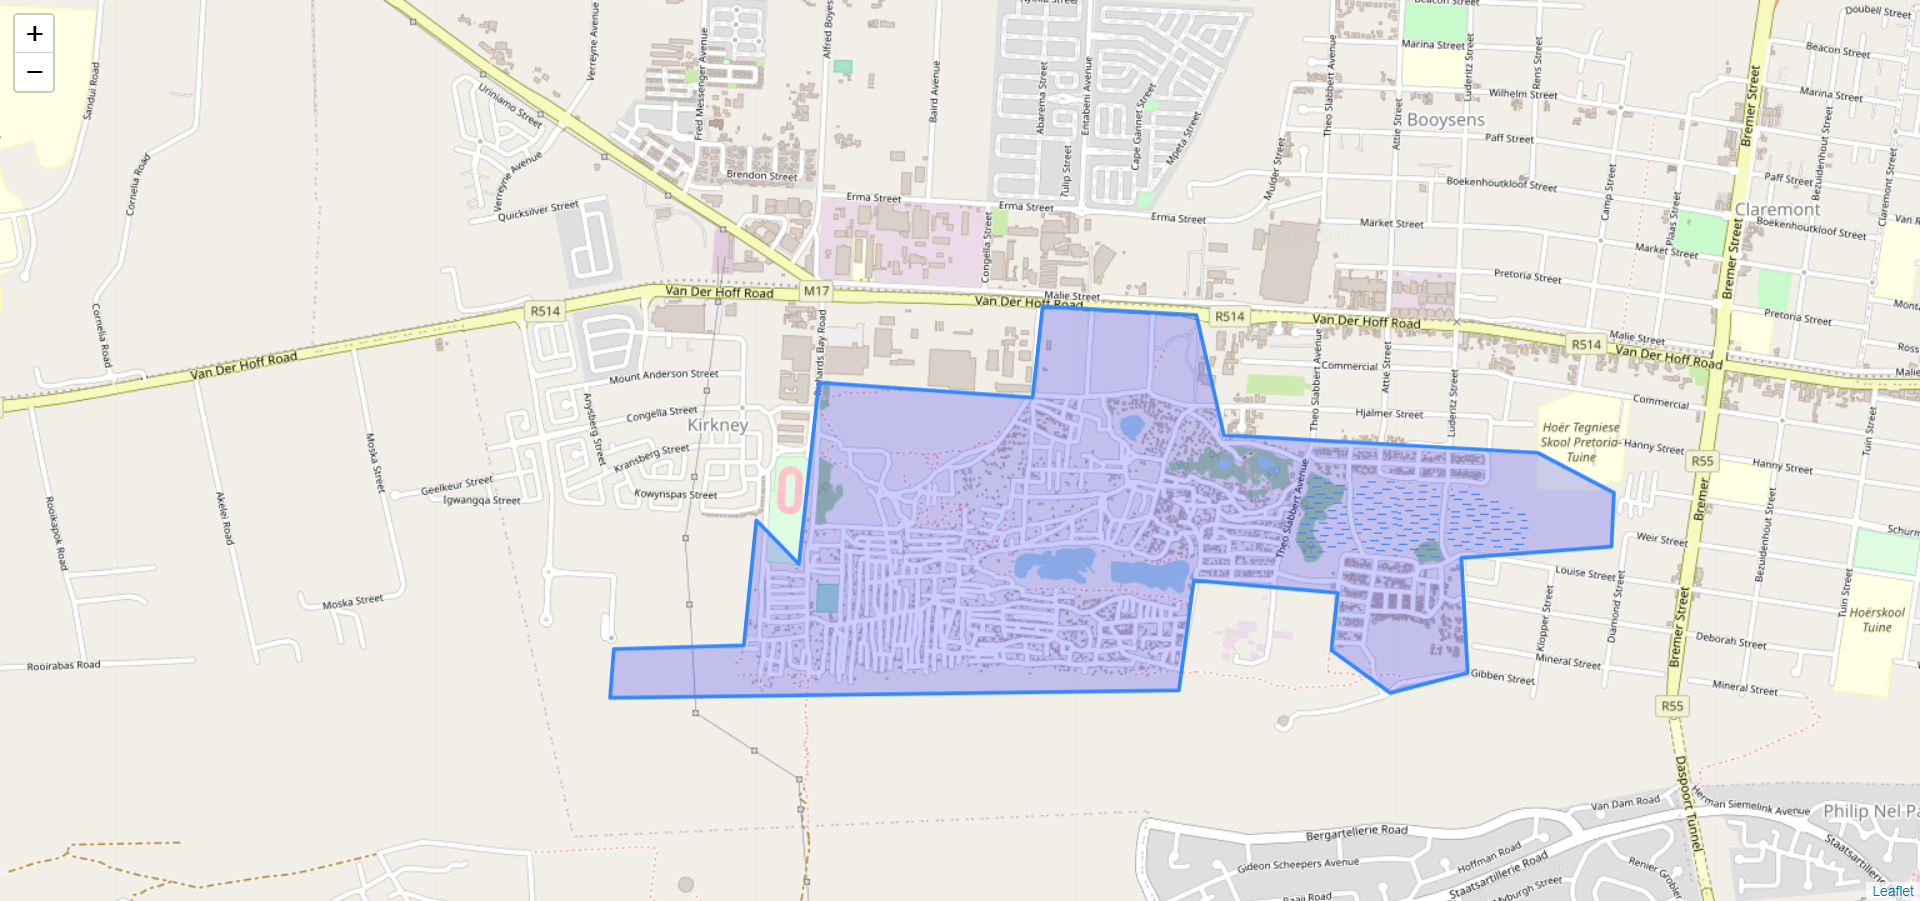
\includegraphics[width=20cm,height=15cm,keepaspectratio]{Figures/Chapter3/Folium}
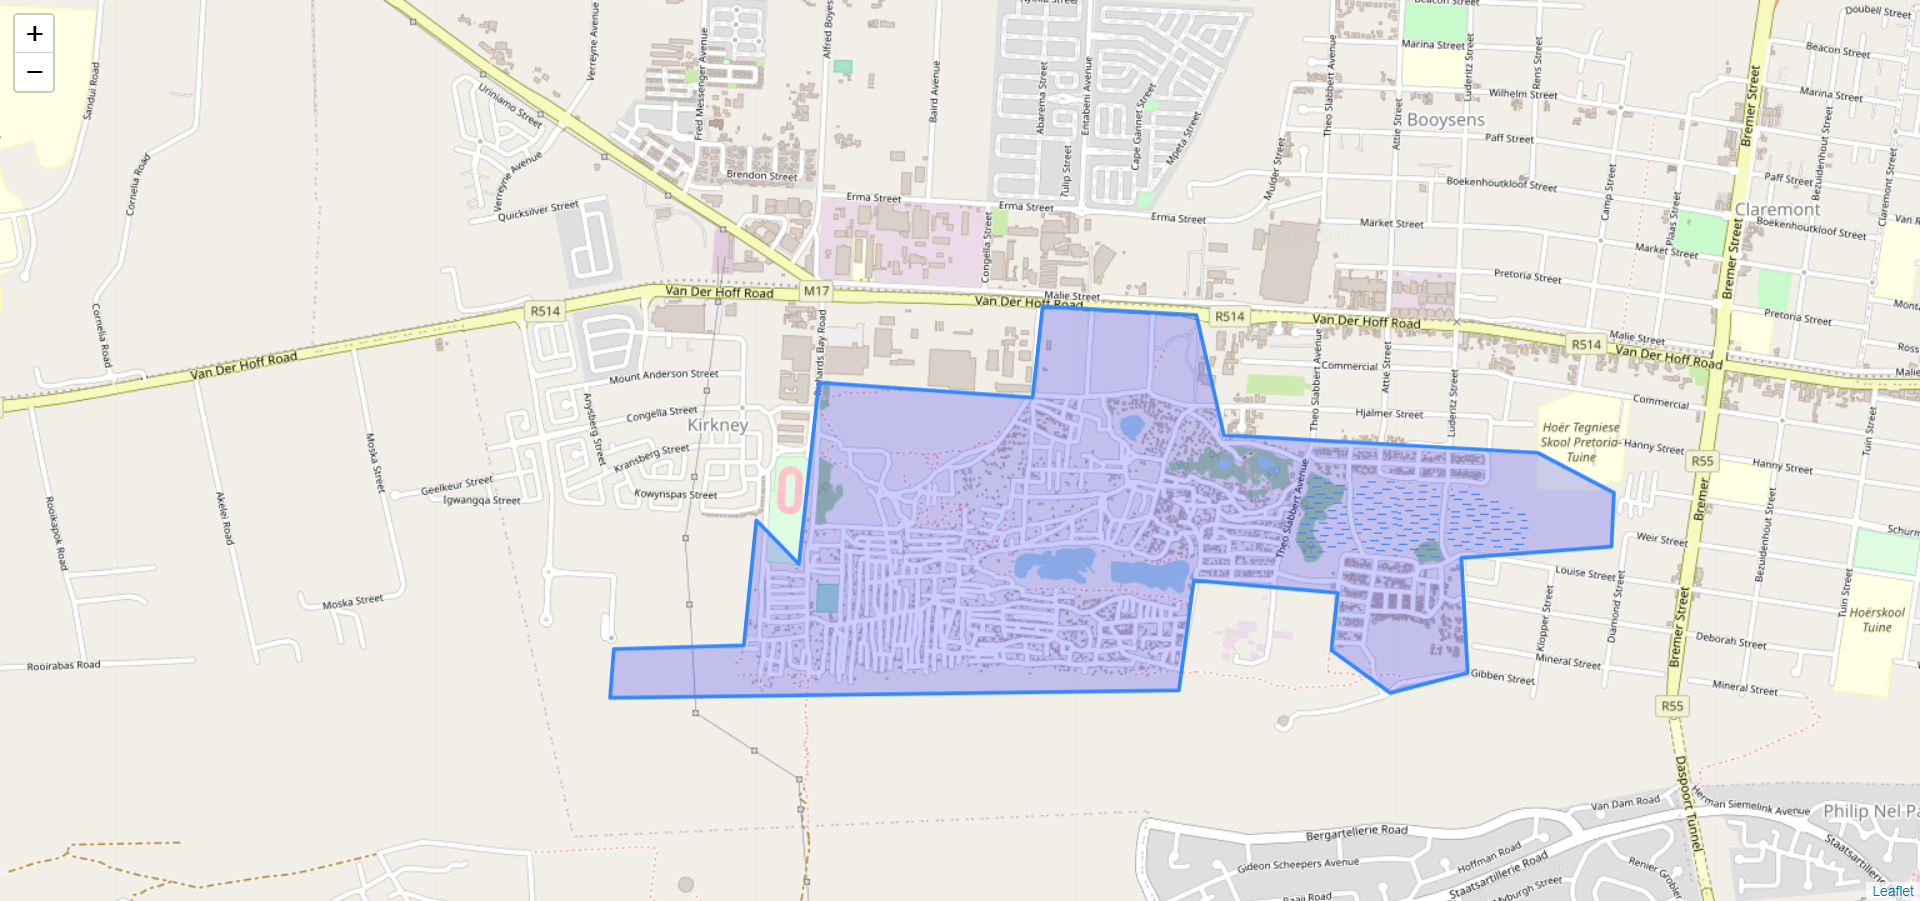
\includegraphics[scale=0.30,angle=90]{Figures/Chapter3/Folium}
\caption{Interactive map of the \textit{Melusi} area}
\label{fig:fol}
\end{figure}
\begin{center}
Source: Own Creation (2021)
\end{center}
\pagebreak
\begin{figure}[H]
\centering
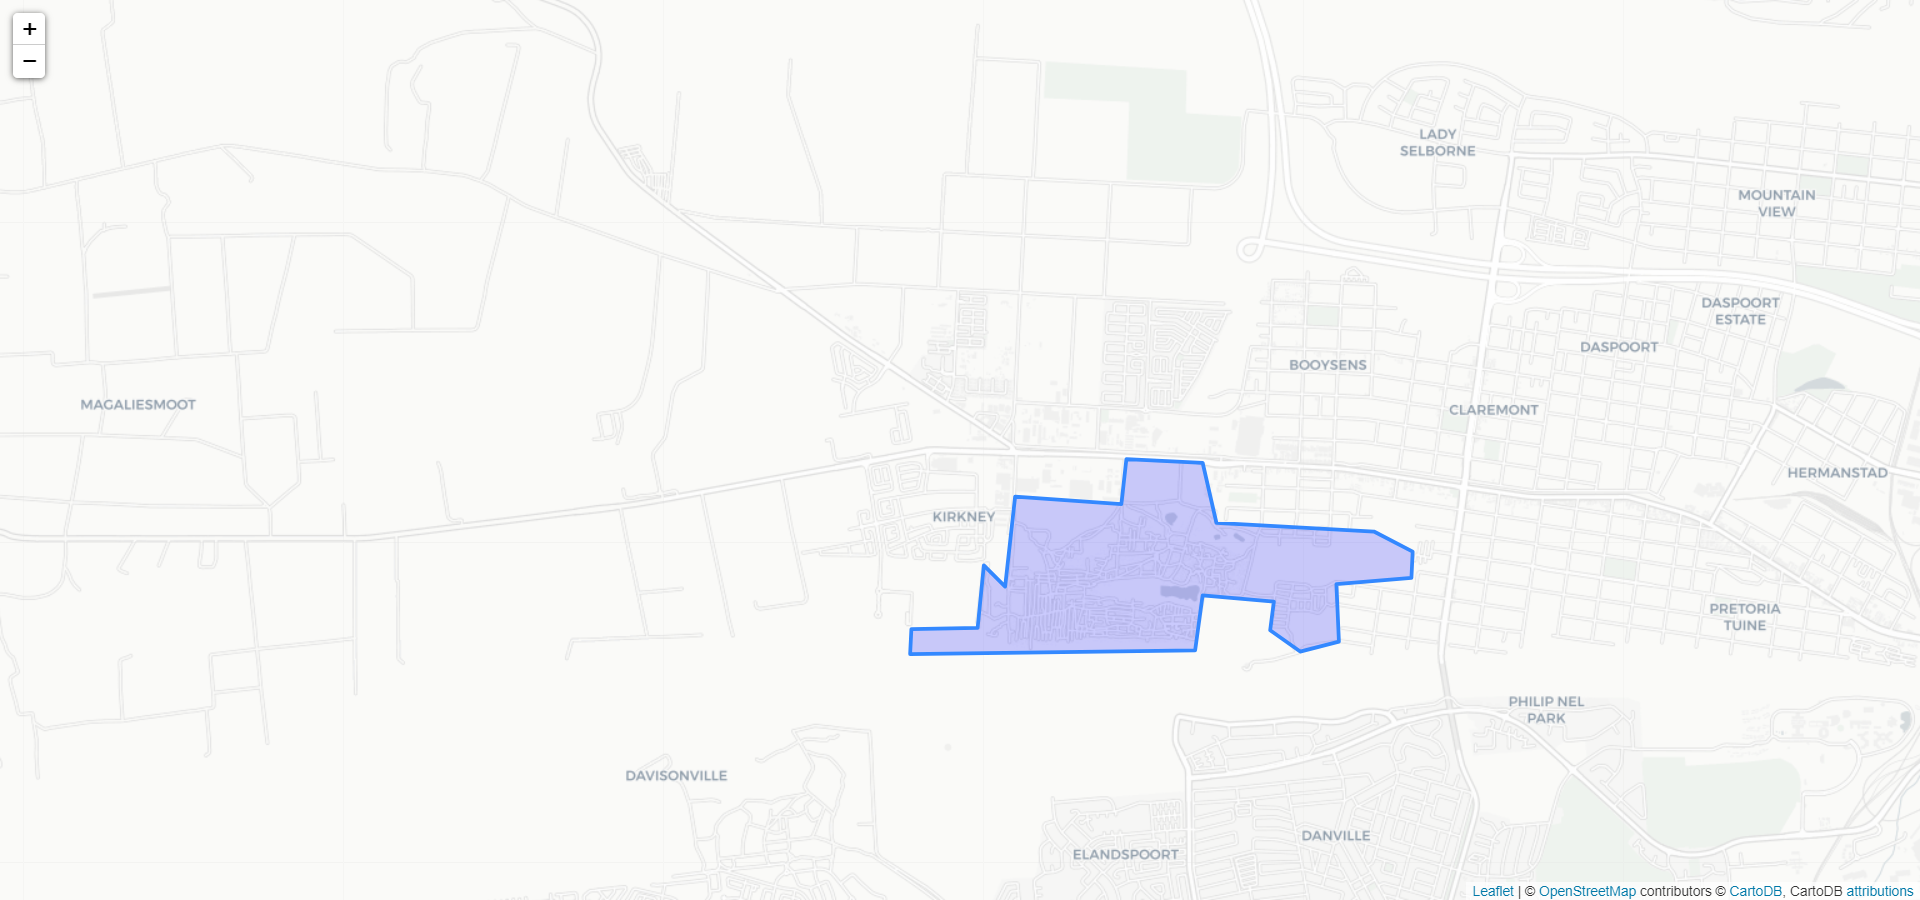
\includegraphics[scale=0.5,angle=90]{Figures/Chapter3/Folium2}
\caption{Another Interactive map of the \textit{Melusi} area}
\label{fig:fol2}
\end{figure}
\begin{center}
Source: Own Creation (2021)
\end{center}
% Chapter 4
\chapter{Results \& Discussion} % Main chapter title
\label{Chapter4} % For referencing the chapter elsewhere, use \ref{Chapter4}
The CA model created in the previous chapter ran for 50 generations or time steps. An image was generated of the simulated Building Based Land Usage growth and it was saved. Additionally, the accuracy of the simulated growth was calculated and saved for each time step. A model without any validation and accuracy testing is ineffectual. For this reason a metric has to be employed to test the accuracy. The metric involved for this process is the Kappa coefficient (also known as Cohen's Kappa coefficient). This metric returns a score that expresses the level of agreement between two annotators and estimate the ground truth. It is utilised vastly in Machine Learning problems, but has also seen its usage in CA urban modelling\cite{m1,m2,m3,m4,m5,m6,m7,m8,m9}. The formula to calculate this coefficient is as follows:\cite{sklearn}
\begin{center}
$\kappa = (p_o - p_e) / (1 - p_e)$
\end{center}
The variable $p_o$ is the the observed agreement ratio (observed accuracy), and the variable $p_e$ is the expected agreement (expected accuracy).

The Table \ref{table:kap} below shows values and their respective magnitudes guidelines for the Kappa coefficient\cite{kappatb}.
\begin{table}[H]
\centering
\caption{Interpreting the Kappa coefficient magnitude}
\label{table:kap}
\begin{tabular}{@{}ll@{}}
\toprule
\multicolumn{1}{l}{Values} & \multicolumn{1}{l}{Magnitude guideline} \\ \midrule
$\kappa \leq 0$                & No agreement                            \\
$0 \leq \kappa \leq 0.20$                     & Slight agreement                        \\
$0.21 \leq \kappa \leq 0.40$                  & Fair agreement                          \\
$0.41 \leq \kappa \leq 0.60$                  & Moderate agreement                      \\
$0.61 \leq \kappa \leq 0.804$                  & Substantial agreement                   \\
$0.81 \leq \kappa \leq 1$                     & Almost perfect agreement                \\ \bottomrule
\end{tabular}
\end{table}
Besides the Kappa coefficient the following additional metrics have been used in similar CA urban modelling research:
\begin{itemize}
\item Visual comparisons between of modelled and real growth\cite{om1,om6,m8}
\item Ratio between modelled urban px and number of real urban px\cite{om2,om5}
\item Regression analysis (r-square values)\cite{om3}
\item The Lee–Sallee index\cite{om4,m1}
\item The Moran's I index\cite{om6}
\item Other spatial indices
\end{itemize}

Besides the Kappa coefficient the the Visual Comparison metric was chosen as an additional metric to validate the accuracy of the final CA model. For this approach two separate techniques were utilised. The first involved creating a GIF image from all the images that were saved during the duration of the CA model execution. The GIF was created using imgflip\footnote{\url{https://imgflip.com/gif-maker}}. The GIF can be found at this document GitHub repository.\footnote{\url{https://github.com/AM-ops/Hons-Project-Documentation/blob/main/Hons-Project-Documentation-Final/Figures/gifs/Growth.gif}} A few snippets from the GIF image are displayed below in Figure \ref{fig:gen50}.
\begin{figure}[H]
\begin{subfigure}{.5\textwidth}
  \centering
  
\includegraphics[width=1\linewidth]{Figures/Chapter4/generation-0-melusi}
  \caption*{Initial State}
\end{subfigure}
\begin{subfigure}{.5\textwidth}
  \centering
  
\includegraphics[width=1\linewidth]{Figures/Chapter4/generation-1-melusi}
  \caption*{Time step $t = 1$}
\end{subfigure}
\end{figure}

\begin{figure}[H]
\begin{subfigure}{.5\textwidth}
  \centering
  
\includegraphics[width=1\linewidth]{Figures/Chapter4/generation-5-melusi}
  \caption*{Time step $t = 5$}
\end{subfigure}
\begin{subfigure}{.5\textwidth}
  \centering
  
\includegraphics[width=1\linewidth]{Figures/Chapter4/generation-10-melusi}
  \caption*{Time step $t = 10$}
\end{subfigure}
\end{figure}

\begin{figure}[H]
\begin{subfigure}{.5\textwidth}
  \centering
  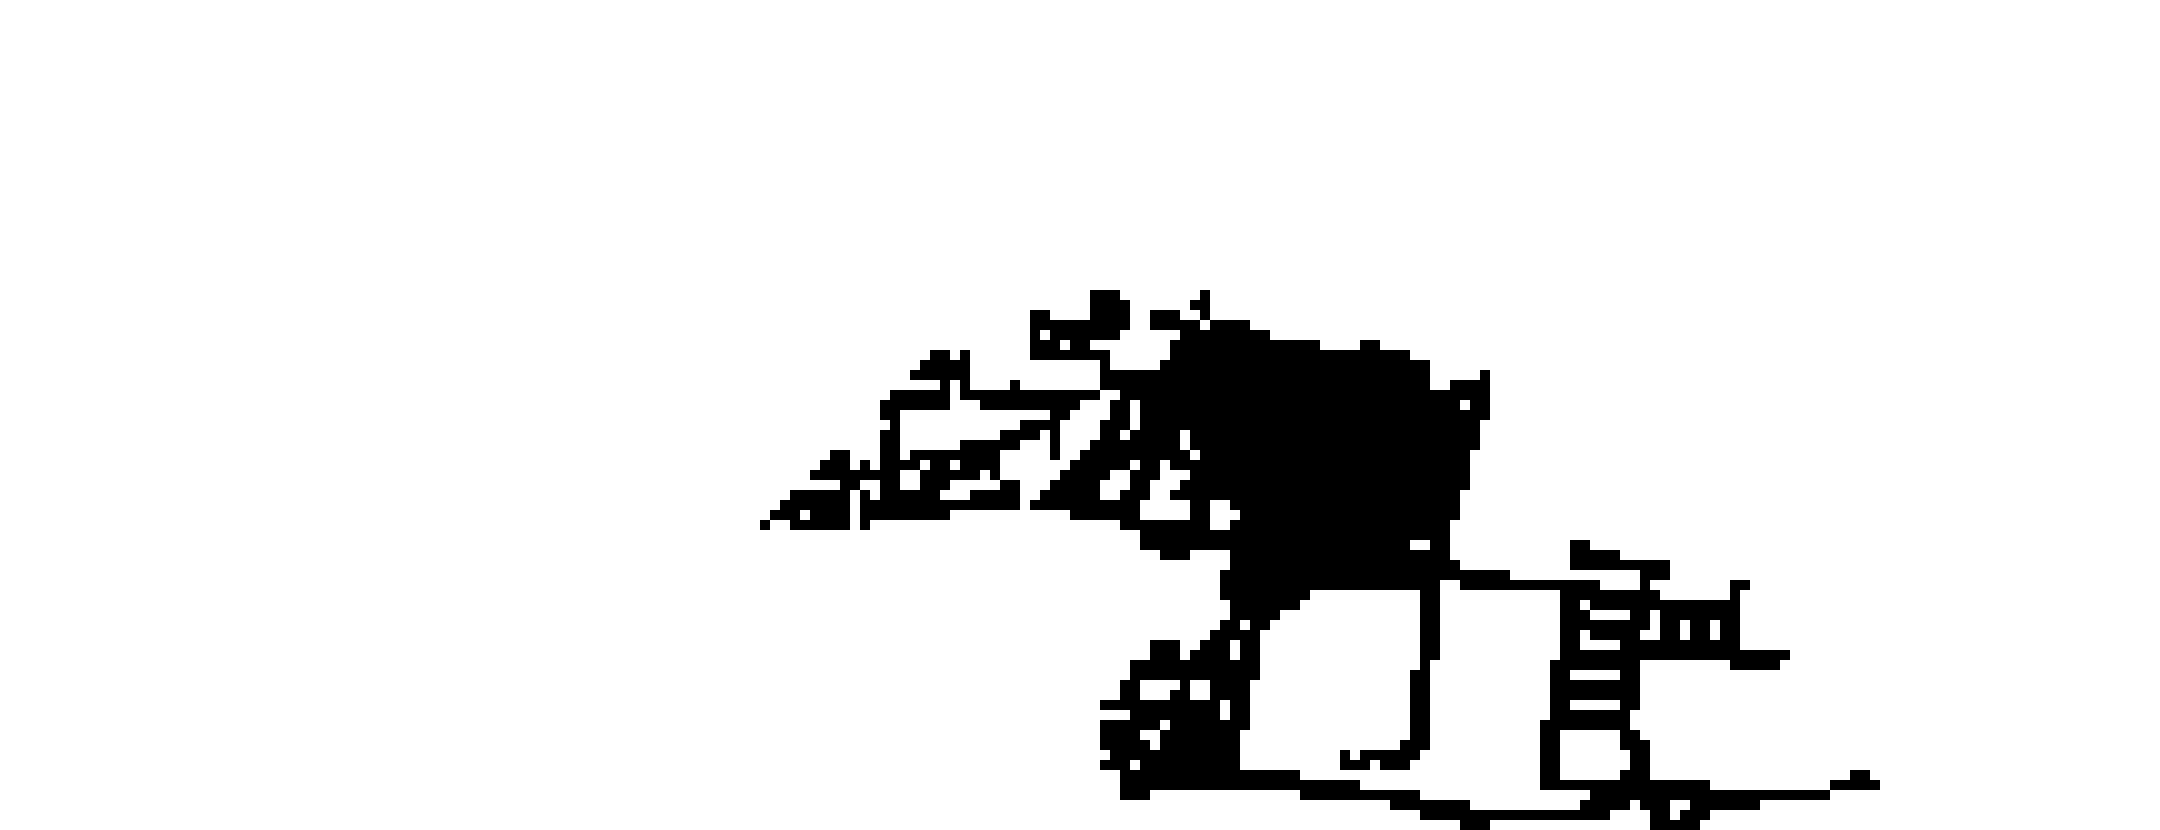
\includegraphics[width=1\linewidth]{Figures/Chapter4/generation-15-melusi}
  \caption*{Time step $t = 15$}
\end{subfigure}
\begin{subfigure}{.5\textwidth}
  \centering
  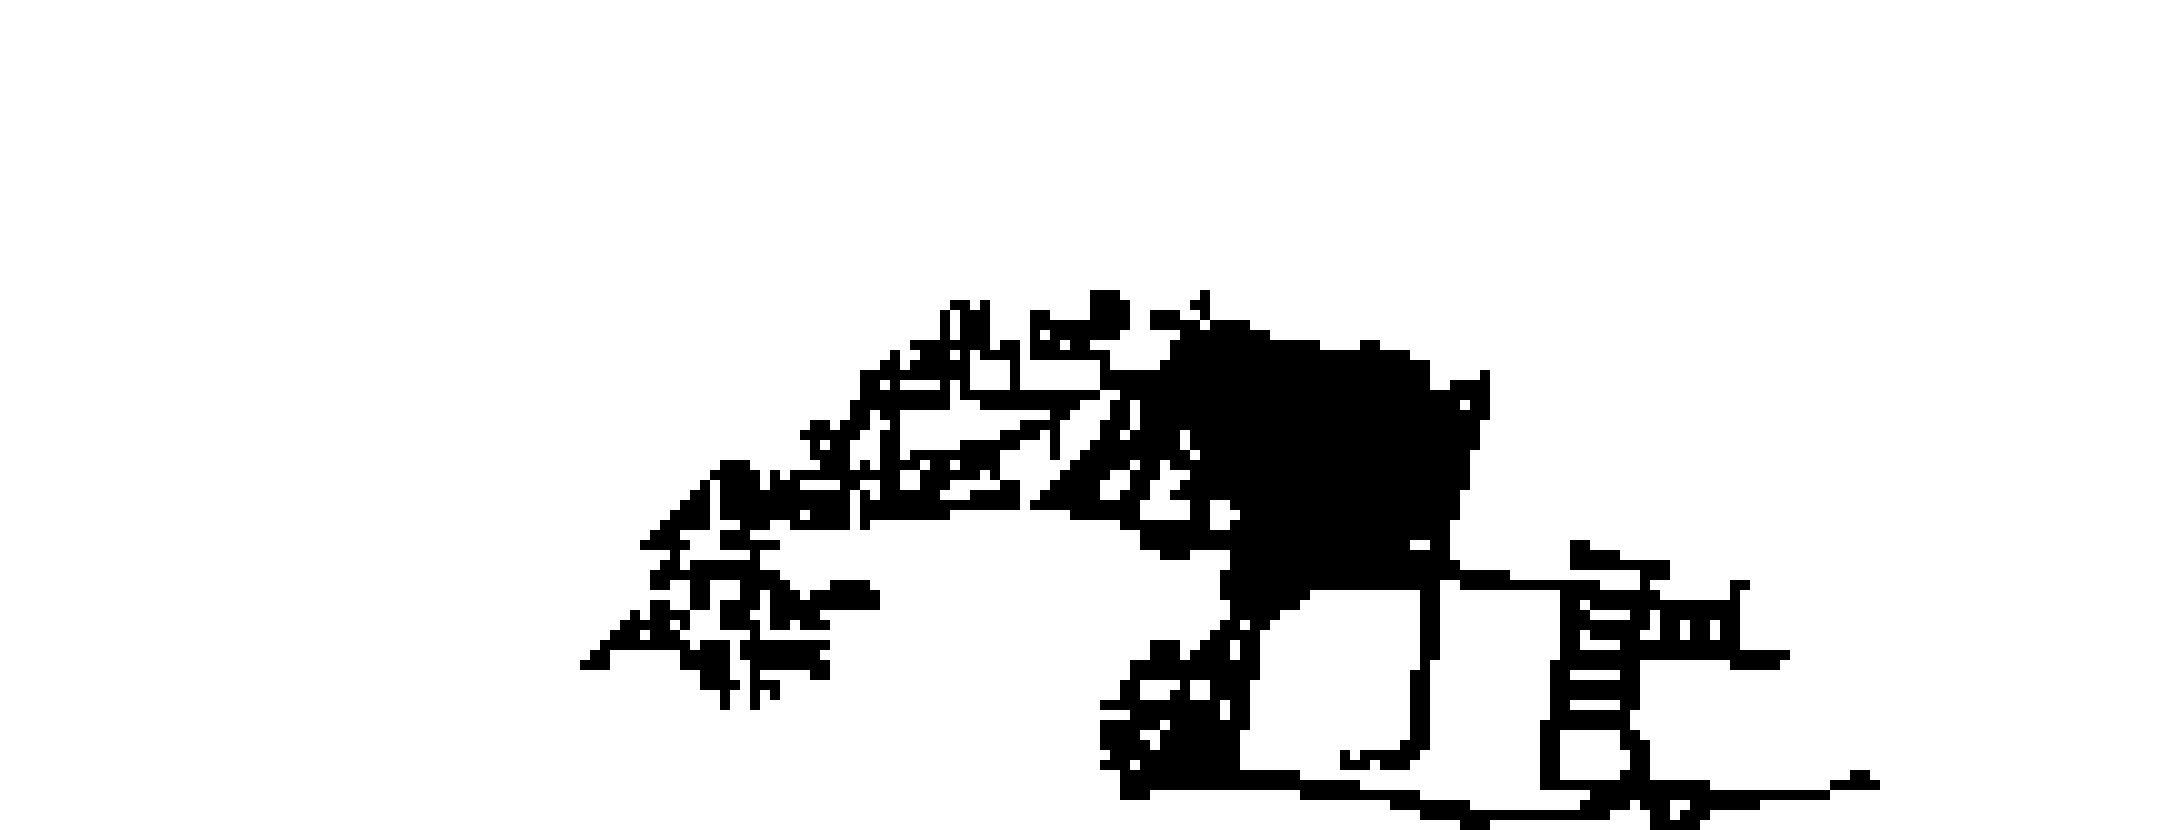
\includegraphics[width=1\linewidth]{Figures/Chapter4/generation-20-melusi}
  \caption*{Time step $t = 20$}
\end{subfigure}
\end{figure}

\begin{figure}[H]
\begin{subfigure}{.5\textwidth}
  \centering
  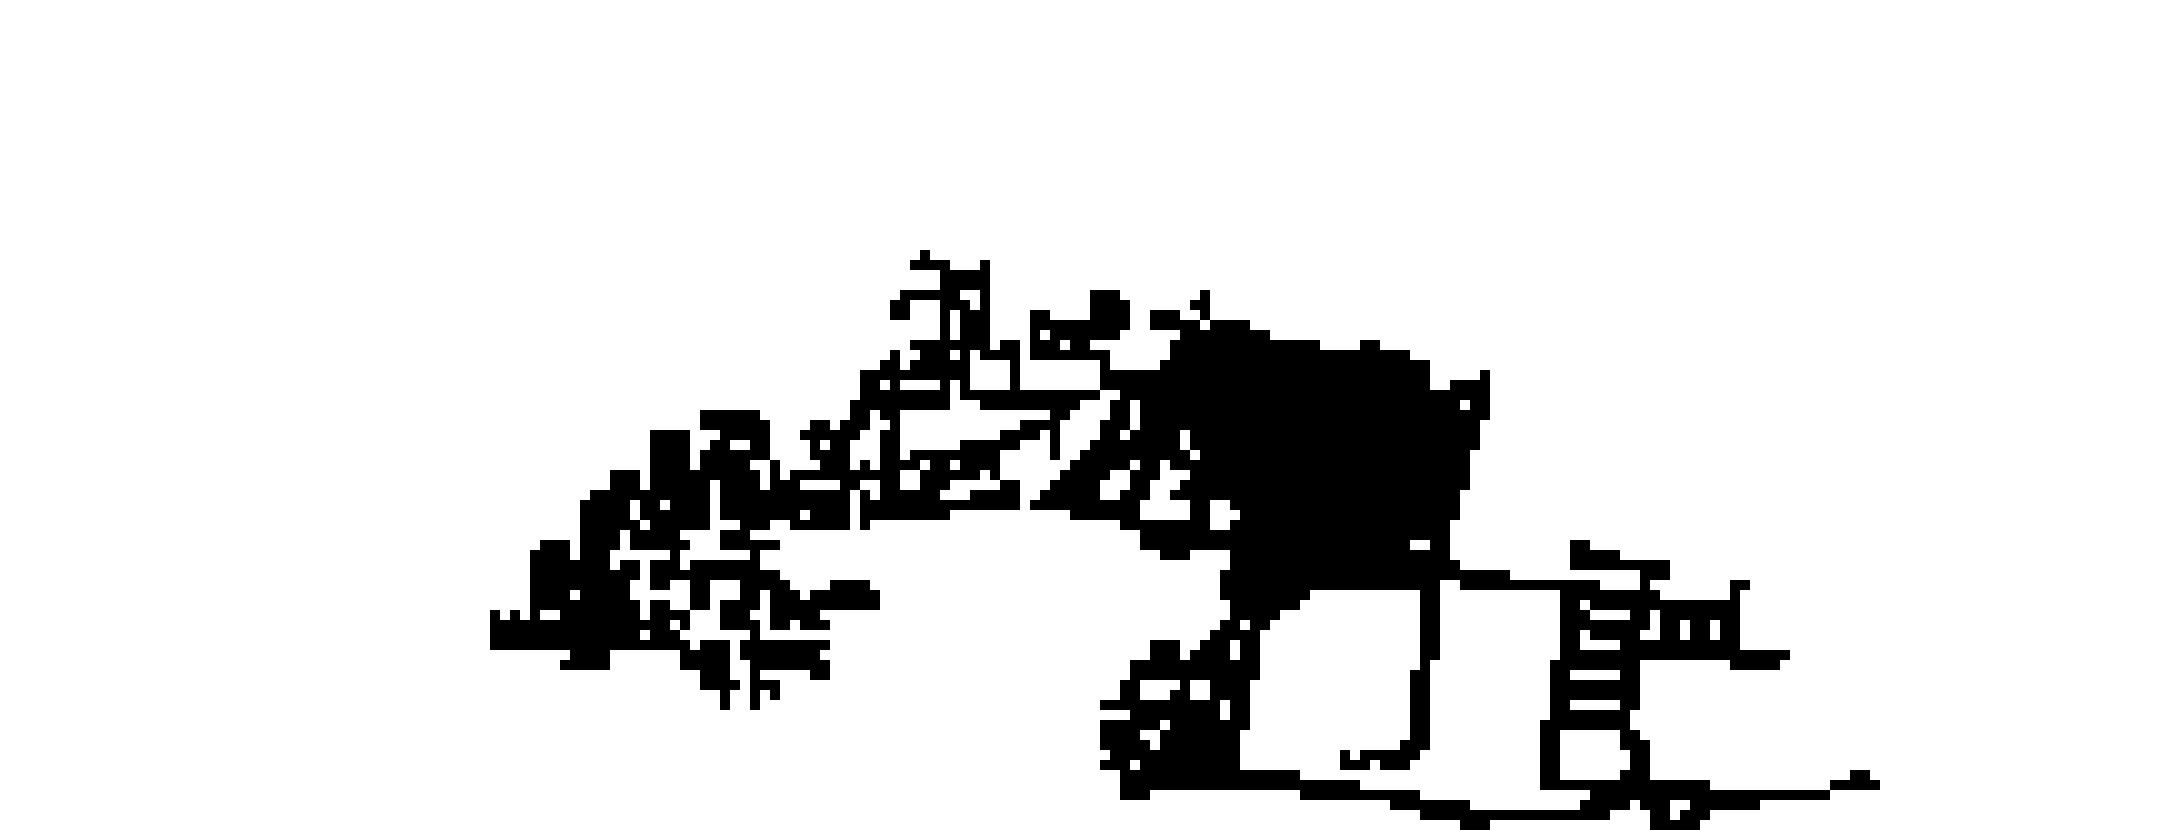
\includegraphics[width=1\linewidth]{Figures/Chapter4/generation-25-melusi}
  \caption*{Time step $t = 25$}
\end{subfigure}
\begin{subfigure}{.5\textwidth}
  \centering
  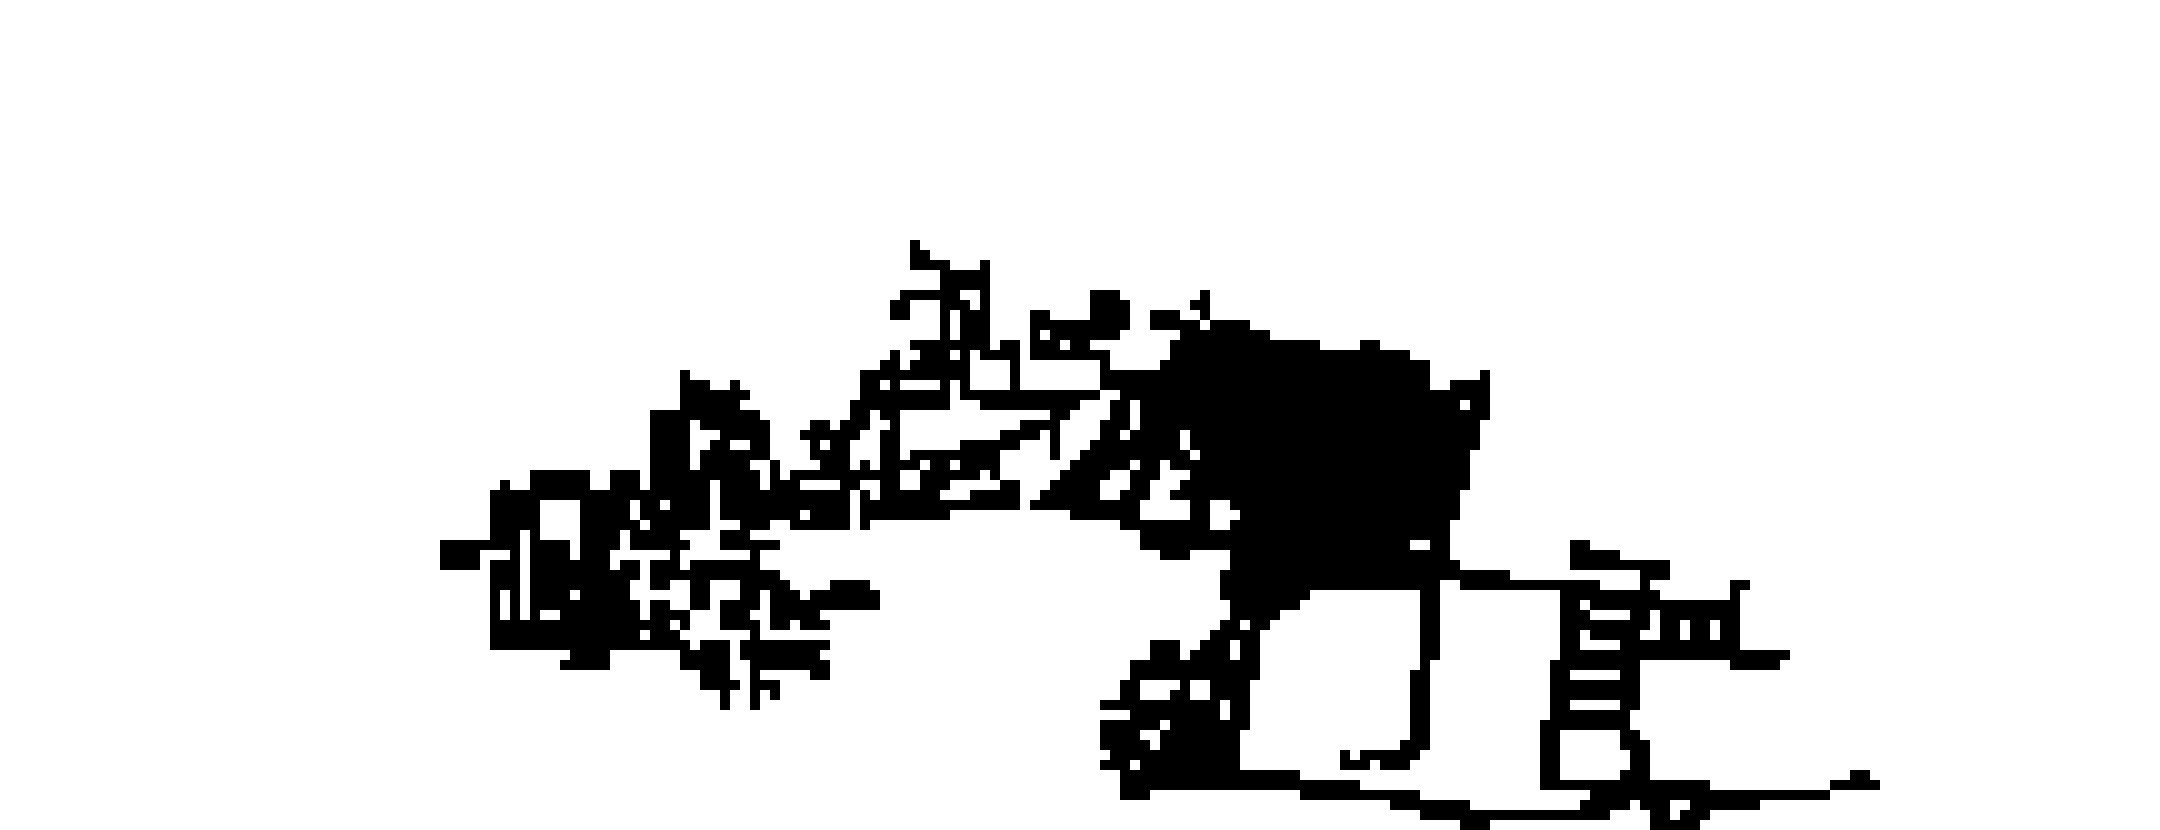
\includegraphics[width=1\linewidth]{Figures/Chapter4/generation-30-melusi}
  \caption*{Time step $t = 30$}
\end{subfigure}
\end{figure}

\begin{figure}[H]
\begin{subfigure}{.5\textwidth}
  \centering
  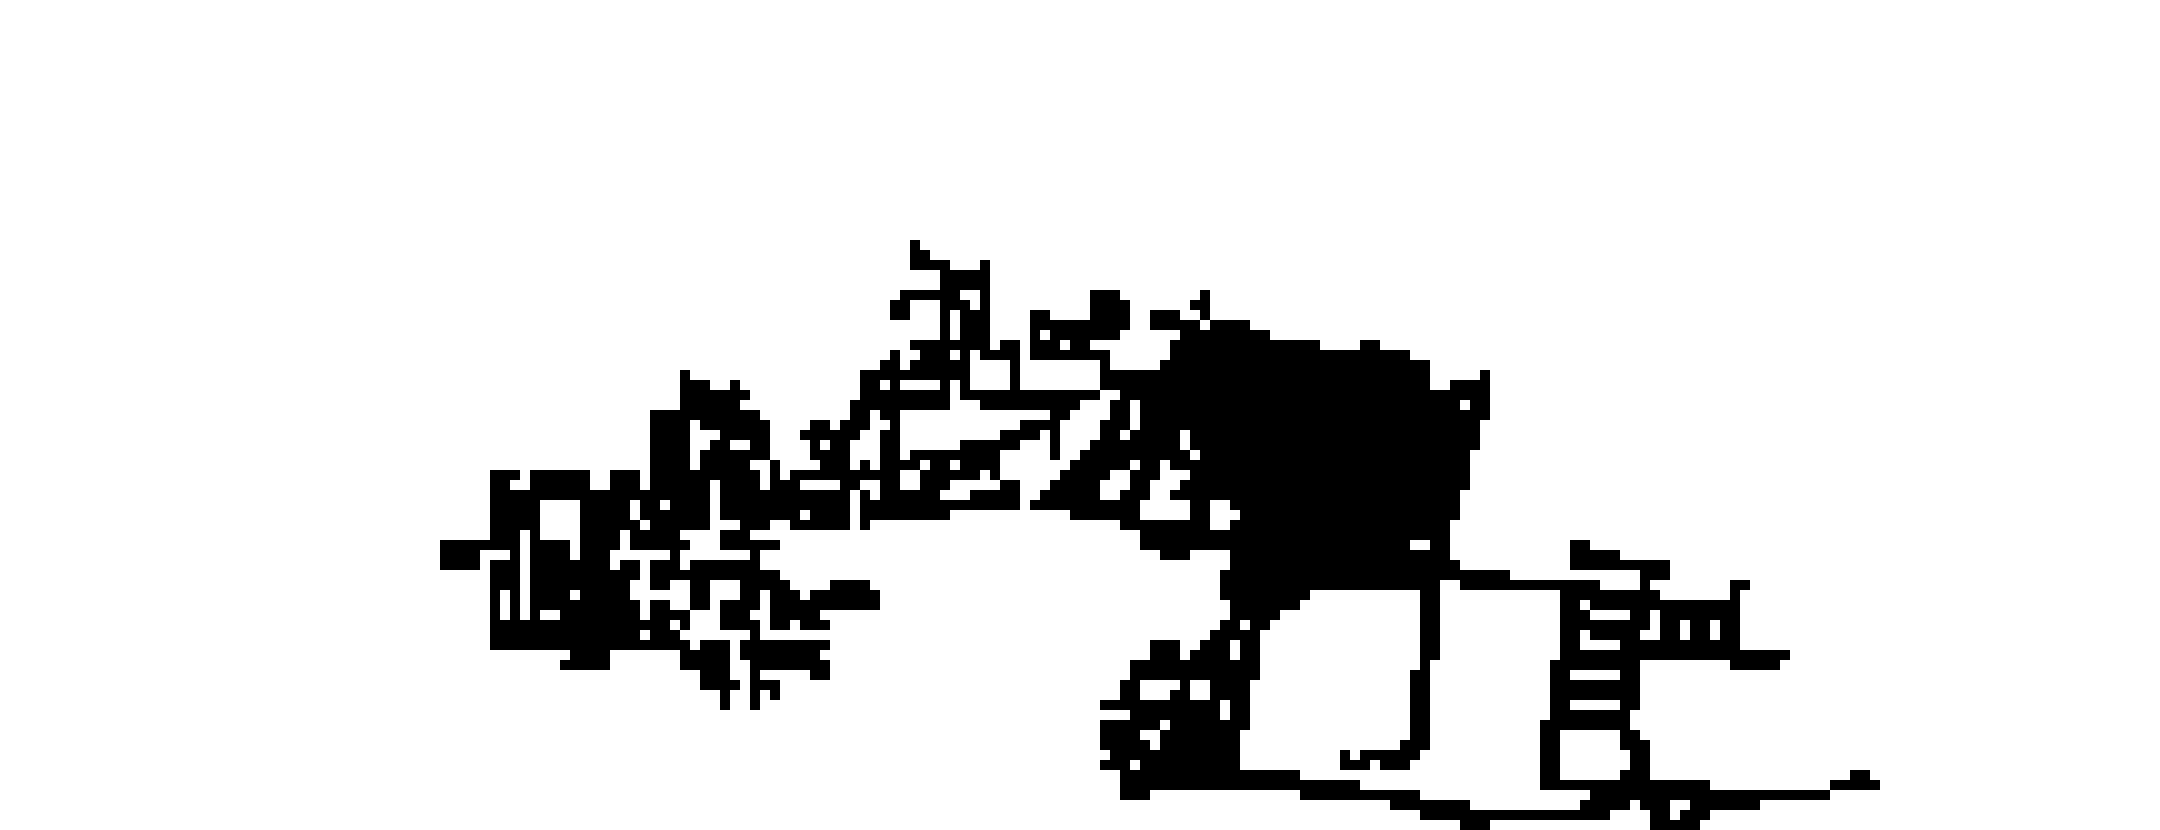
\includegraphics[width=1\linewidth]{Figures/Chapter4/generation-35-melusi}
  \caption*{Time step $t = 35$}
\end{subfigure}
\begin{subfigure}{.5\textwidth}
  \centering
  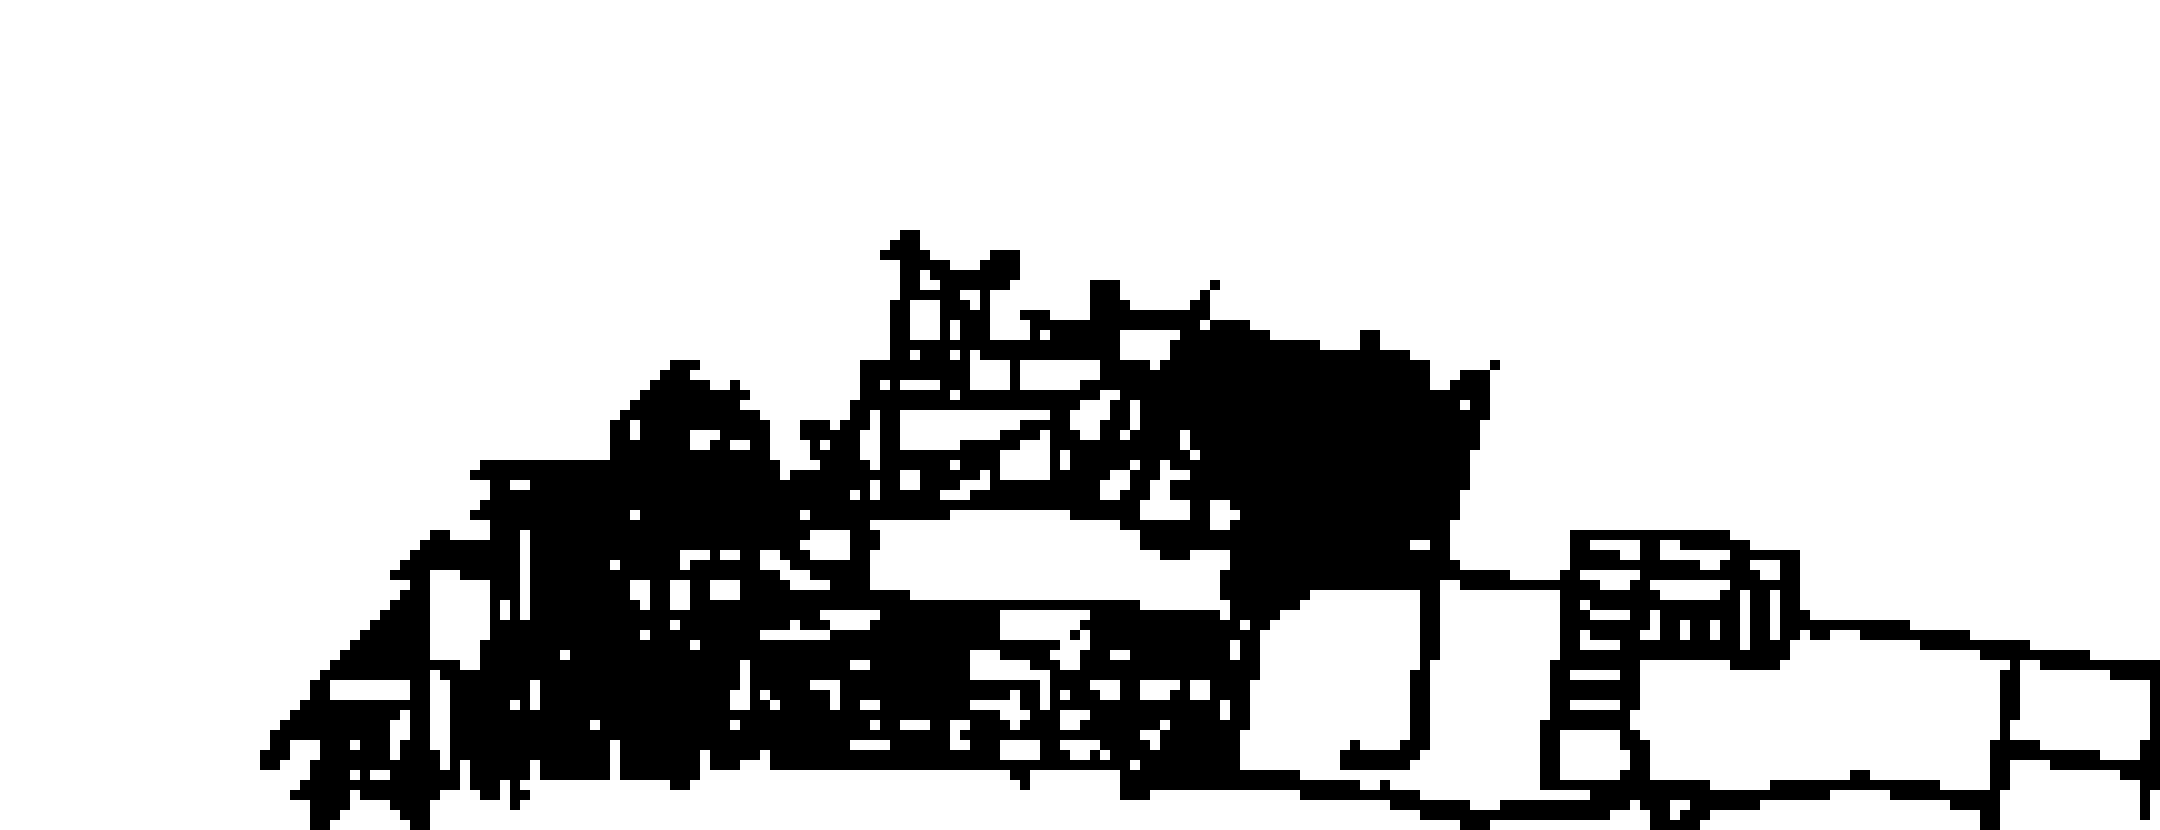
\includegraphics[width=1\linewidth]{Figures/Chapter4/generation-40-melusi}
  \caption*{Time step $t = 40$}
\end{subfigure}
\end{figure}

\begin{figure}[H]
\begin{subfigure}{.5\textwidth}
  \centering
  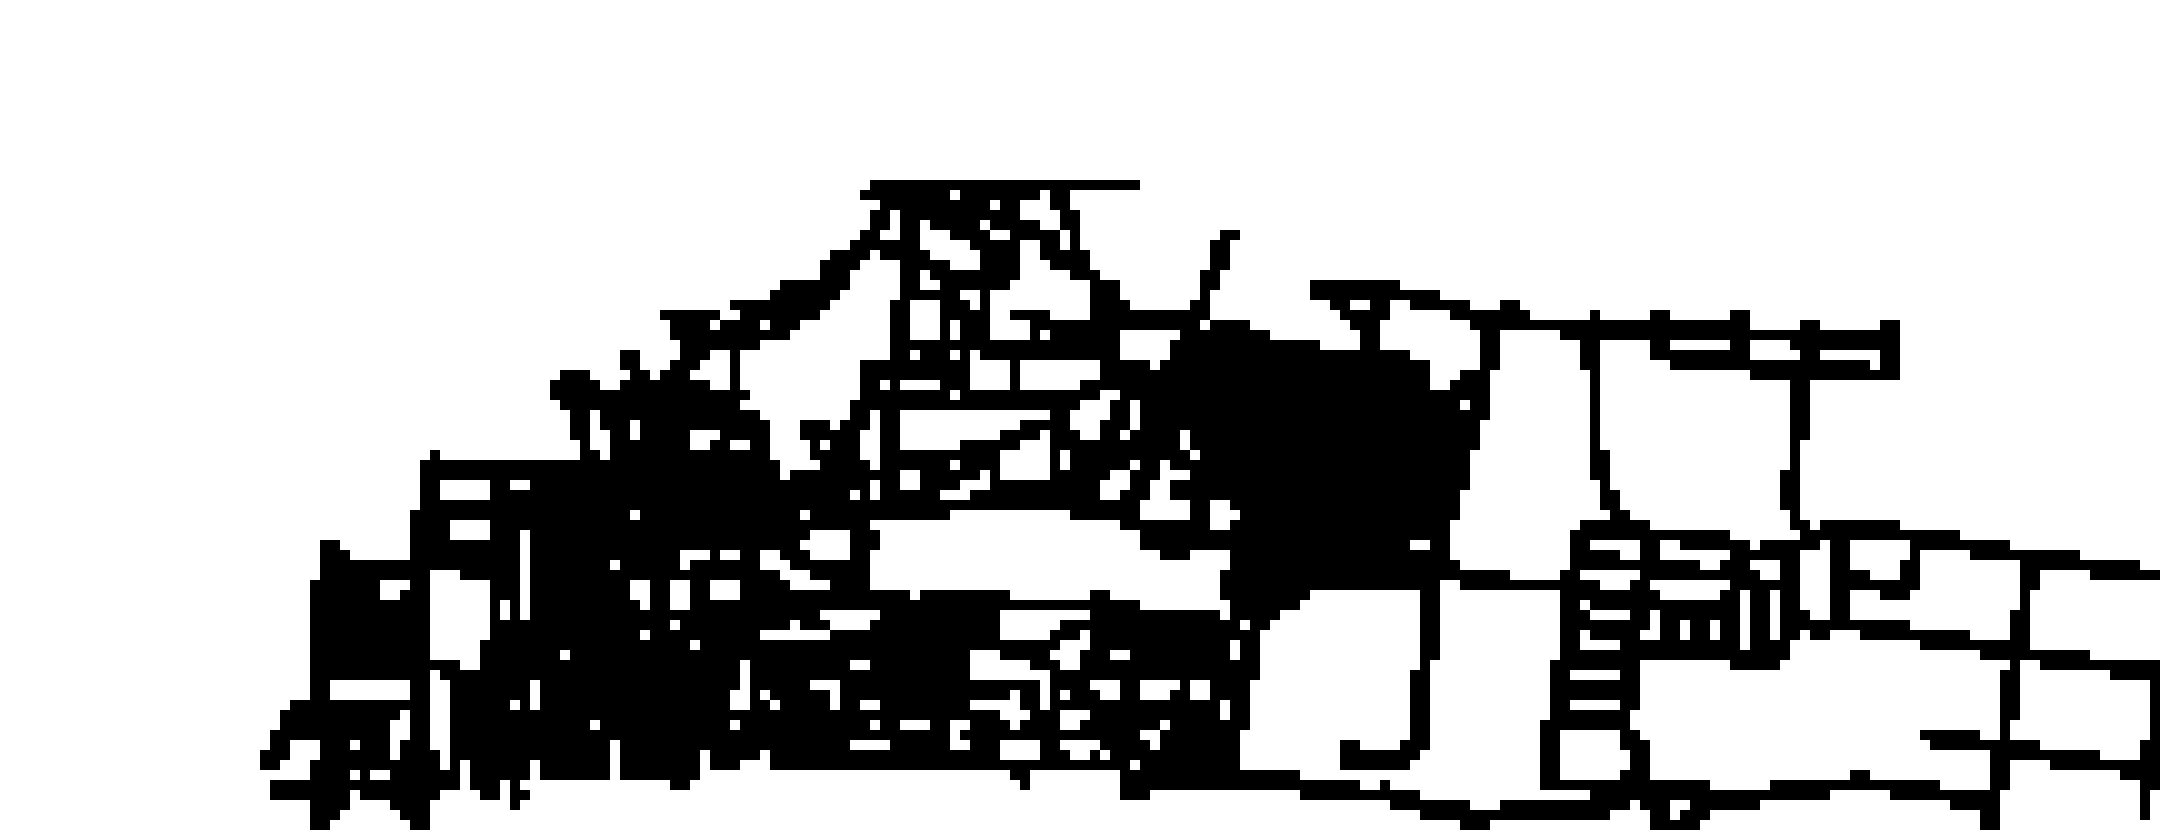
\includegraphics[width=1\linewidth]{Figures/Chapter4/generation-45-melusi}
  \caption{Time step $t = 45$}
\end{subfigure}
\begin{subfigure}{.5\textwidth}
  \centering
  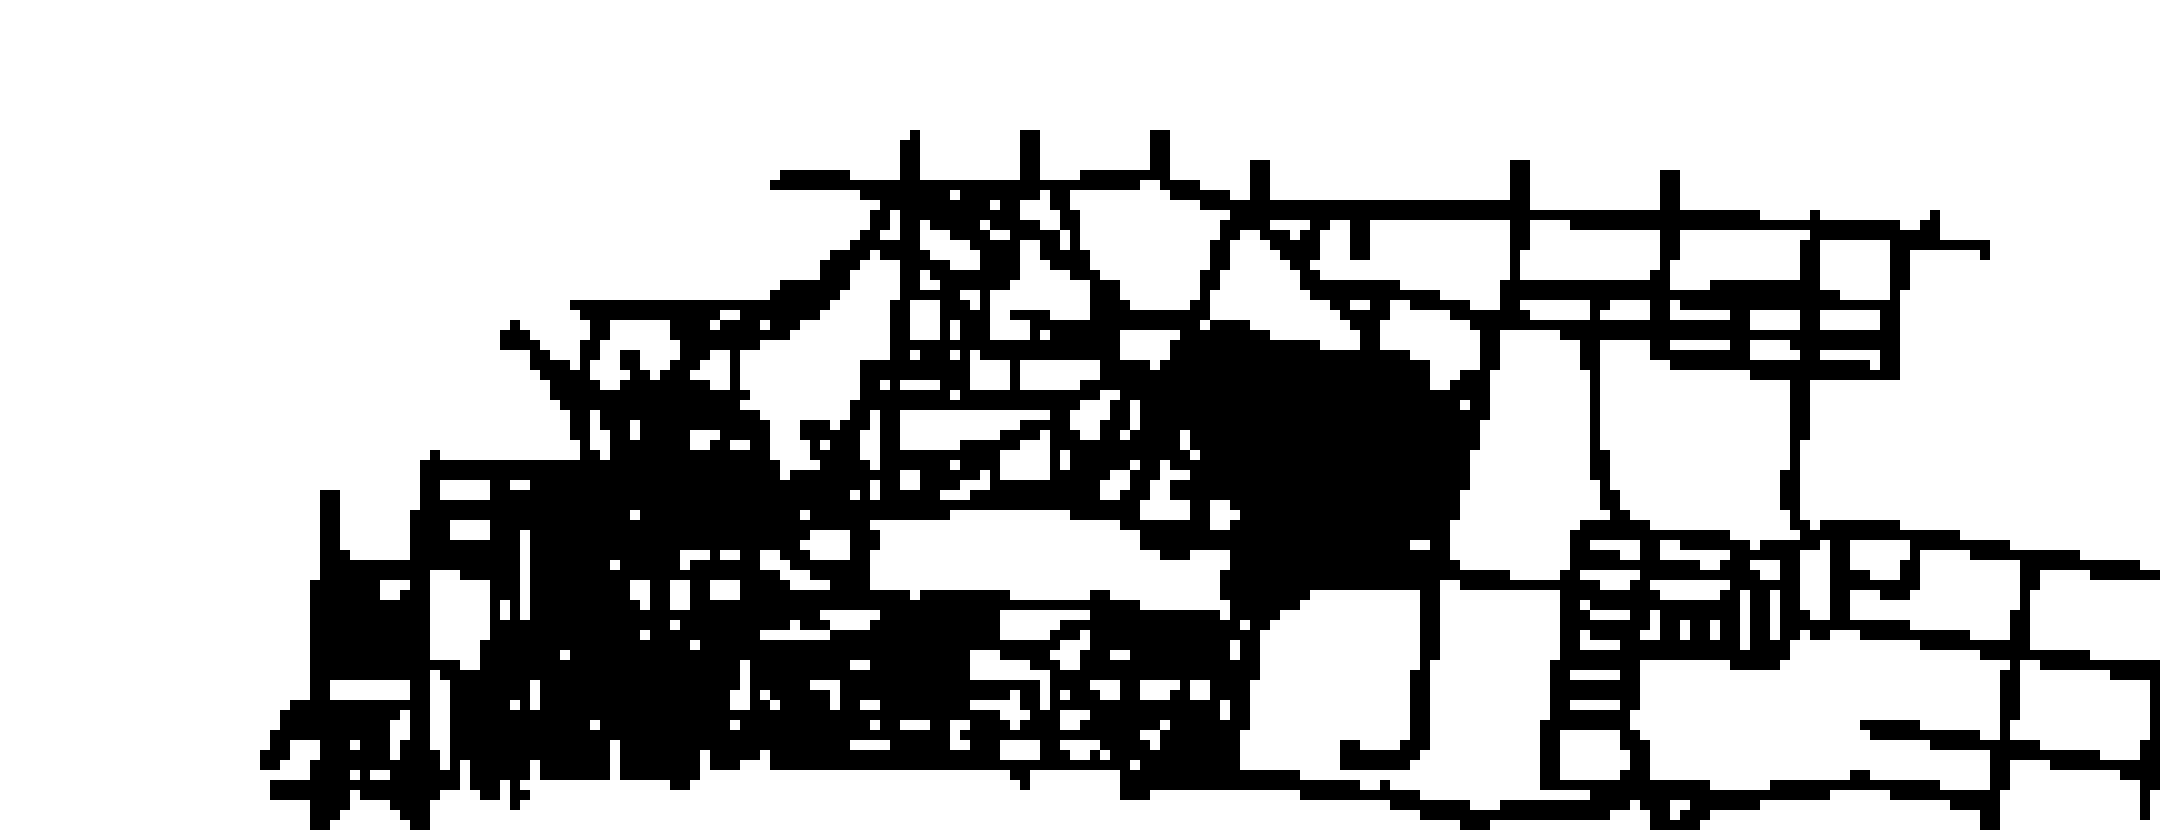
\includegraphics[width=1\linewidth]{Figures/Chapter4/generation-50-melusi}
  \caption{Time step $t = 50$}
\end{subfigure}
\caption{Simulated Growth of Building Based Land Usage for 50 time steps}
\label{fig:gen50}
\end{figure}
\begin{center}
Source: Own Creation (2021)
\end{center}
The second approach in the Visual comparisons metric was to create two images.
\begin{enumerate}
\item An image that overlays the Simulated Growth of the Building Based Land Usage on top of a General Reference Map.
\item An image that overlays the Actual or Existing Building Based Land Usage on top of a General Reference Map.
\end{enumerate}
The images for the above are seen in Figures \ref{fig:simmap} and \ref{fig:curmap} respectively. The validity of the CA model was then seen visually.
\\\\
Going back to the Kappa coefficient, a graph and a table was created to visualise the performance of the CA model over the 50 time steps. The former is seen in Figure \ref{fig:scores} and the later in Table \ref{table:kap2}.

The highest coefficient acieved was at the time step 45
\begin{figure}[H]
\centering
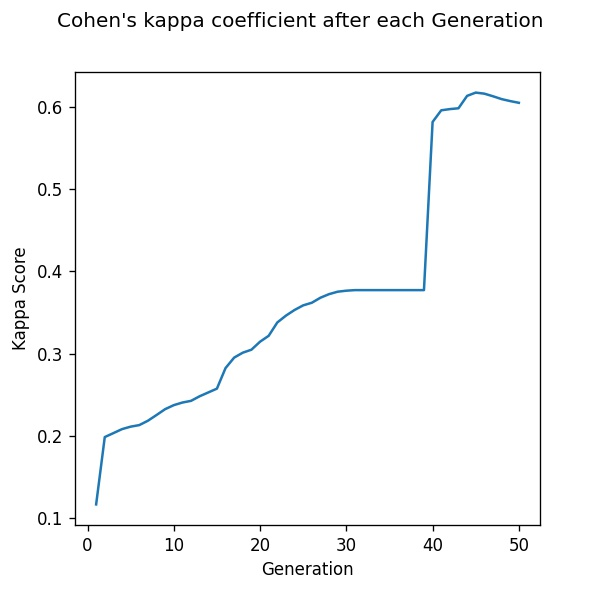
\includegraphics[scale=0.7]{Figures/Chapter4/scoresFigure}
\caption{Kappa coefficient for each Time step simulated}
\label{fig:scores}
\end{figure}

\begin{figure}[H]
\centering
\includegraphics[scale=0.3,angle=90]{Figures/Chapter4/Simulated}
\caption{Simulated Growth of Building Based Land Usage on a Map}
\label{fig:simmap}
\end{figure}

\begin{figure}[H]
\centering
\includegraphics[scale=0.3,angle=90]{Figures/Chapter4/Actual}
\caption{Existing Building Based Land Usage on a Map}
\label{fig:curmap}
\end{figure}



\begin{table}[H]
\setlength{\tabcolsep}{12pt}
\renewcommand{\arraystretch}{1.1}
    \caption{Accuracy results for each time step}
    \label{table:kap2}
    \begin{minipage}{.5\linewidth}
      %\caption{}
            \begin{tabular}{@{}cl@{}}
            \toprule
            Time step & $\kappa$ coefficient \\ \midrule
            1 &  0.11625181498059378 \\
2 &  0.19824922121107136 \\
3 &  0.20306283544626080 \\
4 &  0.20793481429046645 \\
5 &  0.21093437785824343 \\
6 &  0.21283046681369622 \\
7 &  0.21812986043325577 \\
8 &  0.22511088417746883 \\
9 &  0.23225494066337948 \\
10 & 0.23712807908806854 \\
11 & 0.24030784142599682 \\
12 & 0.24236259441785502 \\
13 & 0.24795555301338124 \\
14 & 0.25260419032659376 \\
15 & 0.25724181362747820 \\
16 & 0.28227924369204370 \\
17 & 0.29504157655474317 \\
18 & 0.30102906854032363 \\
19 & 0.30464884852311600 \\
20 & 0.31438848428890310 \\
21 & 0.32157142237699610 \\
22 & 0.33780443805206917 \\
23 & 0.34613948926327110 \\
24 & 0.35302831352863406 \\
25 & 0.35866215860009740 \\ \bottomrule
        \end{tabular}
    \end{minipage}%
    \begin{minipage}{.5\linewidth}
        %\caption{}
        \begin{tabular}{@{}cl@{}}
          \toprule
          Time step & $\kappa$ coefficient \\ \midrule
          26 & 0.36182388889416850 \\
          27 & 0.36795669505675166 \\ 
          28 & 0.37232518280926630 \\
          29 & 0.37529002091648256 \\
          30 & 0.37650949057057026 \\
          31 & 0.37720597829276714 \\
          32 & 0.37720597829276714 \\
          33 & 0.37720597829276714 \\
          34 & 0.37720597829276714 \\
          35 & 0.37720597829276714 \\
          36 & 0.37720597829276714 \\
          37 & 0.37720597829276714 \\
          38 & 0.37720597829276714 \\
          39 & 0.37720597829276714 \\
          40 & 0.58197245681417580 \\
          41 & 0.59617325191136350 \\
          42 & 0.59765374964576660 \\
          43 & 0.59865025952753870 \\
          44 & 0.61375538510117190 \\
          \textcolor{Green}{\textbf{45}} & \textcolor{Green}{\textbf{0.61775529641454560}} \\
          46 & 0.61644571800015240 \\
          47 & 0.61328585200053230 \\
          48 & 0.60982488474318350 \\
          49 & 0.60740162003478520 \\
          50 & 0.60532388693353810 \\ \bottomrule
      \end{tabular}
      %\vspace*{0.8in}
    \end{minipage}
\end{table} 
% Chapter 5

\chapter{Reflection} % Main chapter title

\label{Chapter5} % For referencing the chapter elsewhere, use \ref{Chapter5}

%----------------------------------------------------------------------------------------
%	BIBLIOGRAPHY
%----------------------------------------------------------------------------------------

\printbibliography[heading=bibintoc]

%----------------------------------------------------------------------------------------

%----------------------------------------------------------------------------------------
%	THESIS CONTENT - APPENDICES
%----------------------------------------------------------------------------------------

\appendix % Cue to tell LaTeX that the following "chapters" are Appendices

% Include the appendices of the thesis as separate files from the Appendices folder
% Uncomment the lines as you write the Appendices

% Appendix A

\chapter{Test 1} % Main appendix title

\label{AppendixA} % For referencing this appendix elsewhere, use \ref{AppendixA}

\section{Hello world?}
Test one two three

% Appendix B

\chapter{Research Proposal} % Main appendix title

\label{AppendixB} % For referencing this appendix elsewhere, use \ref{AppendixB}
\begin{minipage}{\textwidth}
\includepdf[scale=0.85,pages=1,offset=0 -4cm]{Proposal.pdf}
\end{minipage}
\includepdf[pages=2- ,pagecommand={}, offset=0 -3cm]{Proposal.pdf}
% Appendix C

\chapter{Code} % Main appendix title

\label{AppendixC} % For referencing this appendix elsewhere, use \ref{AppendixC}
\end{document}  
